\documentclass[a4paper,10pt]{article}

\usepackage[T1]{fontenc}
\usepackage{xltxtra}
\usepackage[francais]{babel}
\usepackage{fancyhdr}

\usepackage{epsfig}
\usepackage{calc}
\usepackage{url}
\usepackage{boxedminipage}

\usepackage{titlesec}
%Pour enlever cette merde de chapter!
%\titleformat{\chapter}[hang]{\bf\huge}{\thechapter}{2pc}{}
\usepackage{graphicx}
%\usepackage{svg}
\usepackage{xcolor}
\usepackage{float}

\usepackage{tabularx}
\usepackage[colorlinks=true, linkcolor=black, citecolor=violet, urlcolor=blue]{hyperref}
\usepackage[sort, authoryear]{natbib}
\usepackage{subcaption}
\bibpunct{[}{]}{,}{n}{,}{,}

% --------------------------------
%Pour compiler sur Ubuntu
%\usepackage[latin1]{inputenc}

% --------------------------------
%Pour compiler sur Manjaro        
\usepackage[utf8]{inputenc}
\usepackage{algorithmicx}
\usepackage{algpseudocode}

% --------------------------------
% Fonction of available fonts
%\usepackage{fontspec} 
%\setmainfont{Adobe Garamond Pro}       
%\setmainfont{EB Garamond}

%% \renewcommand*\rmdefault{ppl}
% --------------------------------

%\usepackage[language=french]{csquotes}

\setcounter{page}{1}
\pagenumbering{Roman}
%%\onehalfspacing

%%%%%%%%%%%%%%%%%%%%%%%%%%%%%%%%%%%%%%%%%%%%%%%%%%%%%%%%%%%
%%%%%%%%%%%%%%%%%%%%%%%%%%%%%%%%%%%%%%%%%%%%%%%%%%%%%%%%%%%
%% Définitions à personnaliser 

%% Pour les noms, utilisez la première lettre du prénom suivi du 
%% nom de famille (première lettre majuscule, reste en minuscule).


%%%% Indiquer le nom de l'encadrant ci-dessous:

\def\nomEncad{Martin \textsc{Quinson}}

%% Si le projet est co-encadré indiquer les deux noms à la suite dans 
%% Le même champs


%%%% Indiquer les noms des étudiants participant ci-dessous:

\def\nomEtudA{Louisa \textsc{Bessad}}

%% Si le projet est encadré par moins de 4 étudiants laissez
%% les variables inutiles vides


%%%% Indiquer la référence (numero) et le nom du sujet ci-dessous:

\def\refProjet{Numéro Projet} 
\def\titreProjetCourt{Titre court}
\def\titreProjetLong{Real-time online emulation of real applications on SimGrid with Simterpose}

%% Le titre court ne doit pas faire plus d'une vingtaine de caractère
%% résumez le à quelques mots essenciels


%%%% Indiquer le type de document et sa version ci-dessous:

\def\typeDoc{Pré-rapport}
 
%% - Rapport intermédaire
%% - Rapport final

%\let\origsec\section
%\renewcommand{\section}[1]{\newpage\origsec{#1}}



%%%%%%%%%%%%%%%%%%%%%%%%%%%%%%%%%%%%%%%%%%%%%%%%%%%%%%%%%%%
%%%%%%%%%%%%%%%%%%%%%%%%%%%%%%%%%%%%%%%%%%%%%%%%%%%%%%%%%%%
%% Définitions à ne pas modifier
 
%%%% ||| Mise en page verticale ||| 
\setlength{\voffset}{-1in} % a4:reste 297mm pour les 5 suivants:
\setlength{\topmargin}{15mm}         % avant l'en-tête
\setlength{\headheight}{20mm}        % hauteur de l'en-tête 
\setlength{\headsep}{10mm}            % entre l'en-tête et le corps
\setlength{\textheight}{220mm}       % hauteur du corps
\setlength{\footskip}{12mm}          % pied de page par rapport au corps 
%\setlength{\footlength}{2em}

%%%%% --- Mise en page horizontale ---
\setlength{\hoffset}{-1in} % a4:reste 210mm 
\setlength{\oddsidemargin}{25mm}     % entre hoffset et le corps
\setlength{\evensidemargin}{25mm}    % entre hoffset et le corps
\setlength{\marginparwidth}{0mm}     % largeur de la marge
\setlength{\marginparsep}{0mm}       % séparateur corps marge
\setlength{\textwidth}{160mm}        % largeur du corps

%\usepackage{fullpage}
%\setlength{\headheight}{20mm}        % hauteur de l'en-tête 
%\setlength{\headsep}{10mm}            % entre l'en-tête et le corps
%\setlength{\textheight}{200mm}
%\setlength{\footskip}{0mm}          % pied de page par rapport au corps 

\def\annee{2015}



%%%%%%%%%%%%%%%%%%%%%%%%%%%%%%%%%%%%%%%%%%%%%%%%%%%%%%%%%%%
%% Début du document

\begin{document}
\begin{titlepage}

\newcommand{\HRule}{\rule{\linewidth}{0.5mm}} % Defines a new command for the horizontal lines, change thickness here

\center % Center everything on the page
 
%----------------------------------------------------------------------------------------
%	HEADING SECTIONS
%----------------------------------------------------------------------------------------

\textsc{\LARGE Université Pierre et MArie Curie}\\[0.44cm] % Name of your university/college
\textsc{\Large Master informatiqe}\\[0.44cm] % Major heading such as course name
\textsc{\large Systèmes et Applications Répartis}\\[1.44cm] % Minor heading such as course title

\textsc{\LARGE Loria}\\[0.44cm] % Name of your university/college
\textsc{\Large Equipe VERIDIS}\\[1.44cm] % Major heading such as course name

%----------------------------------------------------------------------------------------
%	TITLE SECTION
%----------------------------------------------------------------------------------------

\HRule \\[0.4cm]
{ \huge \bfseries Real-time online emulation of real applications on SimGrid with Simterpose}\\[0.4cm] % Title of your document
\HRule \\[1.44cm]
 
%----------------------------------------------------------------------------------------
%	AUTHOR SECTION
%----------------------------------------------------------------------------------------

\begin{minipage}{0.4\textwidth}
\begin{flushleft} \large
\emph{Etudiant:}\\
Louisa \textsc{Bessad} % Your name
\end{flushleft}
\end{minipage}
~
\begin{minipage}{0.4\textwidth}
\begin{flushright} \large
\emph{Encadrant} \\
Martin \textsc{Quinson} % Supervisor's Name
\\\vspace{1.44cm} \emph{Rapporteur:} \\ Sébastien
\textsc{Monnet}
\end{flushright}
\end{minipage}\\[2cm]

% If you don't want a supervisor, uncomment the two lines below and remove the section above
%\Large \emph{Author:}\\
%John \textsc{Smith}\\[3cm] % Your name

%----------------------------------------------------------------------------------------
%	DATE SECTION
%----------------------------------------------------------------------------------------

{\large \today}\\[3cm] % Date, change the \today to a set date if you want to be precise

%----------------------------------------------------------------------------------------
%	LOGO SECTION
%----------------------------------------------------------------------------------------

%\includegraphics{Logo}\\[1cm] % Include a department/university logo - this will require the graphicx package

\includegraphics[scale=0.2]{Pictures/png/UPMC_sorbonne.png}\hspace{3cm}

\includegraphics[scale=0.1]{Pictures/loria_logo.jpg}

%----------------------------------------------------------------------------------------

\vfill % Fill the rest of the page with whitespace
\end{titlepage}
\clearpage
%\vfill

%%\newpage
%%\mbox{}
%%\newpage

%%%%%%%%%%%%%%%%%%%%%%%%%%%%%%%%%%%%%%%%%%%%%%%%%%%%%%%%%%%
%% Définition des en-têtes et pied de pages
\pagestyle{fancyplain}
%\fancyhead{}
%\fancyfoot{}
%
\fancyhead[L]{\textsc{Université Pierre et Marie Curie} \\ {\color{white} b} \\ \nomEtudA}
\fancyhead[C]{\textbf{Pré-rapport}}%\\\titreProjetCourt}}
\fancyhead[R]{\textsc{LORIA} \\ {\color{white} b} \\ \nomEncad}

\fancyfoot[L]{
\includegraphics[width=3cm]{Pictures/png/UPMC_sorbonne.png}}
\fancyfoot[C]{\textbf{\thepage}}
\fancyfoot[R]{
\includegraphics[width=4cm]{Pictures/loria_logo.jpg}}

%\lhead[\fancyplain{}{\texttt{Université Pierre et Marie Curie}\\
%          Master Informatique\\ UE \textbf{PSAR} fév. \annee \\ \nomEncad}]
%      {\fancyplain{}{\textsc{Université Pierre et Marie Curie}\\
%          Master Informatique\\ UE \textbf{PSAR} \annee \\ \nomEncad}}
%\chead[\fancyplain{}{\textbf{Projet \refProjet\\\titreProjetCourt}}]
%      {\fancyplain{}{\textbf{Projet \refProjet\\\titreProjetCourt}}}
%\rhead[\fancyplain{}{\nomEtudA\\\nomEtudB}]
%      {\fancyplain{}{\nomEtudA\\\nomEtudB}}
%\lfoot[\fancyplain{}{\epsfig{figure=UPMC_sorbonne.eps,width=3cm}}]
%      {\fancyplain{}{\epsfig{figure=UPMC_sorbonne.eps,width=3cm}}}
%\cfoot[\fancyplain{}{\textbf{\thepage/\pageref{fin}}}]
%      {\fancyplain{}{\textbf{\thepage/\pageref{fin}}}}
%\rfoot[\fancyplain{}{\typeDoc}]
%      {\fancyplain{}{\typeDoc}}


%%%%%%%%%%%%%%%%%%%%%%%%%%%%%%%%%%%%%%%%%%%%%%%%%%%%%%%%%%%


\tableofcontents
%\vfill
\newpage
%% \mbox{}
%% \newpage

\listoffigures
\newpage
%% \mbox{}
%% \newpage

%Abstract
%\begin{abstract}
 %TODO
  %% Dans le cadre de ce stage nous allons nous intéresser aux applications ditribuées à large échelle et comment on peut les tester et évaluer leurs performances via une combinaison d'émulation et de simulation en utilisant SIMGRID et Simterpose qui sont deux projets européens. SIMGRID a été lancé en 1999 pour étudier des algorithmes d'ordonnancement sur des plateformes hétérogènes dans un environnement distribué et faciliter leur programmation. Il fournit les outils de base nécessaire à la simulation de ce type d'applications. Simterpose s'insère dans le projet SIMGRID afin de pouvoir étudier des applications complètes et pas uniquement leur modèle que l'on fournit habituellement en paramètre au simulateur. Le but est de faire de l'émulation en utilisant un simulateur que sera SIMGRID. Puisque nous nous intéressons aux applications distribuées notre émulateur doit pouvoir\textit{i)} exécuter un grand nombre d'instances d'une même application sur un même système afin de pouvoir debugguer, \textit{ii)} évaluer des applications ayant de nombreuses condition d'exécution (simple n\oe ud, réseau complet), \textit{iii)} collecter les informations concernant l'application pendant qu'elle s'exécute.
%\end{abstract}
%\newpage

{\color{white} blabla} \vspace{7cm}

Ce stage se déroule au Loria, Laboratoire Lorrain de Recherche en Informatique
et ses Applications, unité mixte de recherche commune à plusieurs
établissements: le CNRS, l'INRIA, et l' Université de Lorraine. Le LORIA a pour
mission la recherche fondamentale et appliquée en sciences informatiques et ce,
depuis sa création, en 1997.

L'encadrement est assuré par Martin Quinson au sein de l'équipe VERIDIS, dont les sujets de recherches sont la conception de méthodes pour les systèmes distribués et d'outils pour la vérification et la validation de systèmes.



\newpage

\setcounter{page}{1}
\pagenumbering{arabic}
% Content
%% {\color{white} blabla} \vspace{7cm}


Je voudrais remercier mon tuteur Martin Quinson pour m'avoir permis d'effectuer ce stage, durant lequel j'ai beaucoup appris.

Je tiens également à remercier mon encadrant universitaire Sébastien Monnet pour ses précieux conseils.

%% \newpage
\section{Introduction}

%% intro/objectif: virtualisation légère d'applications distribuées (tester des applications distribuées réelles: test regression et performance, légère car on veut tester des centaines d'instances)

%% Applications: stockage distribué (CEPH, TAHOE/LAFS) et RT event processing (Storm)

Dans le cadre de ce stage, nous allons nous intéresser aux applications
distribuées. Il s'agit d'applications dont une partie ou la totalité des
ressources n'est pas localisée sur la machine où l'application s'exécute, mais
sur plusieurs machines distinctes. Ces dernières communiquent entre elles via le
réseau pour s'échanger les données nécessaires à l'exécution de
l'application. Les applications distribuées ont de nombreux avantages: elles
permettent notamment d'augmenter la disponibilités des données en se les
échangeant, comme les applications Torrent (BitTorrent, $µ$Torrent...). Grâce au
projet BOINC\footnote{\url{https://boinc.berkeley.edu/}} par exemple, on peut
partager la puissance de calcul inutilisée de sa machine. Depuis une dizaine
d'années, la popularité de ces applications distribuées ne cesse de croître. On
peut notamment penser aux applications de stockage de données
LAFS\footnote{\url{https://tahoe-lafs.org/trac/tahoe-lafs}} et
CEPH\footnote{\url{http://ceph.com/}}. La première apporte un stockage robuste
qui préserve les données même si un site est physiquement détruit. La seconde
souhaite fournir performance, fiabilité et scalabilité.  Elles deviennent de
plus en plus complexes avec des contraintes et des exigences de plus en plus
fortes, en particulier au niveau des performances et de l'hétérogénéité des
plateformes et des ressources utilisées. Il est donc de plus en plus
difficile de créer de telles applications (absence d'horloge et mémoire
centrale, deadlock, race, famine) mais aussi de les tester.  En effet, malgré
l'évolution des applications distribuées, les protocoles d'évaluation de leurs
performances n'ont que peu évolués.
\newline

Actuellement, il existe trois façons principales de tester le comportement
d'applications distribuées \citep{gustedt2009experimental}: l'exécution sur
plate-forme réelle, la simulation et l'émulation.

La première solution consiste à exécuter réellement l'application sur un parc de
machines et d'étudier son comportement en conditions réelles. Cela permet de la
tester sur un grand nombre d'environnements. L'outil créé et développé en partie
en France pour cela est \textbf{Grid'5000}\footnote{Infrastructure de 8000 c\oe
  urs répartis dans la France entière crée en
  2005. \\ \url{https://www.grid5000.fr/mediawiki/index.php/Grid5000:Home}}\citep{GRID5000},
un autre outil développé à l'échelle mondiale est
\textbf{PlanetLab} \footnote{Crée en 2002, cette infrastructure de test compte
  aujourd'hui 1340 c\oe urs. \\ \url{http://www.planet-lab.org}}. Néanmoins,
pour mettre en \oe uvre ces solutions complexes, il faut disposer des
infrastructures nécessaires pour effectuer les tests. Il faut également écrire
une application complète capable de gérer toutes ces ressources
disponibles. Enfin, du fait du partage des différentes plateformes entre
plusieurs utilisateurs, les expériences sont difficilement reproductibles.

La seconde solution consiste à faire de la simulation: on modélise ce que l'on
souhaite étudier (application et/ou environnement) via un programme appelé
simulateur. Dans ce cas, pour pouvoir tester des applications distribuées sur un
simulateur, on doit d'abord abstraire l'application ainsi que l'environnement
d'exécution. Pour cela, on identifie les propriétés de l'application et de son
environnement puis on les transforme à l'aide de modèles mathématiques. Ainsi,
on va exécuter dans le simulateur le modèle de l'application et non
l'application réelle, dans un environnement également modélisé. Cette solution
est donc facilement reproductible, plus simple à mette en \oe uvre, et permet de
prédire l'évolution du système étudié grâce à l'utilisation de modèles
mathématiques. De nos jours, les simulateurs tel que
\textbf{SimGrid}\citep{CASANOVA:SimGrid, MARTIN:SimGrid} peuvent simuler des
applications distribuées mettant à contribution des milliers de
n\oe uds. Néanmoins, avec la simulation on ne peut valider qu'un modèle et non
l'application elle-même.

La troisième solution consiste à faire de l'émulation: on exécute réellement
l'application mais dans un environnement virtualisé grâce à un logiciel,
l'émulateur. Ce dernier joue le rôle d'intercepteur pour virtualiser
l'environnement d'exécution.
%On fera ainsi croire à l'application qu'elle s'exécute sur une machine autre que l'hôte.
Cette solution représente un intermédiaire entre la simulation et l'exécution
sur plateforme réelle visant à résoudre les limitations de ces deux
solutions. En effet, les actions de l'application sont réellement exécutées sur
la machine hôte (la machine réelle sur laquelle s'exécute l'émulation) et grâce
à la virtualisation, l'application pense être dans un environnement différent de
la machine réelle. De plus, cela évite d'avoir deux versions de l'application en
terme de code: une pour la simulation et une pour la production. L'émulation
peut-être faite \textit{off-line} (on sauvegarde les actions de l'application
sur disque et on les rejoue plus tard dans un simulateur) ou \textit{on-line}
(on bloque l'application le temps que le temps de réponse de la plateforme
virtualisée soit calculé).

%% Il existe deux types d'émulation pour les applications distribuées; la
%% virtualisation standard et la légère. On parle de virtualisation légère quand on
%% souhaite tester des applications sur une centaine d'instances.

Au cours de ce stage, nous allons nous intéresser plus particulièrement à l'exécution d'applications distribuées arbitraires au dessus de la plateforme de simulation SimGrid. Pour cela, nous allons présenter en section \ref{section:emulation} les méthodes utilisées
pour faire de la virtualisation %% légère: limitation et interception
. Puis en
section \ref{section:sota} nous présenterons les projets permettant de faire de
l'émulation pour tester des applications dans un environnement
distribué. Ensuite, nous expliquerons en section \ref{section:simterpose},
pourquoi dans le cadre du projet Simterpose c'est la virtualisation légère par
interception qui a été choisie et comment elle fonctionne. Pour finir, nous
concluerons en section \ref{section:ccl}.

\newpage
\section{Pourquoi choisir l'émulation simulée}

Il existe trois façons de tester des applications distribuées. La première consiste à exécuter réellement l'application sur un parc de machines et d'étudier le comportement de l'application en temps-réel, ce que fait actuellement \textbf{Grid'5000} {\color{red}mettre citation}. Néanmoins pour mettre en \oe uvre cette solution complexe il faut disposer des architectures nécessaires pour effectuer les tests. De part le partage des différentes plateformes entre divers utilisateurs les expériences ne sont pas forcément reproductibles. Une deuxième solution consiste à simuler l'exécution des applications à l'aide d'un simulateur tel que \textbf{SIMGRID} {\color{red}mettre citation}. On doit alors modéliser l'application ainsi que l'environnements d'exécution grâce à des modèles mathématiques. Le problème avec la simulation est que l'on exécute pas vraiment l'application, on ne peut alors valider qu'un modèle et pas l'application puisqu'on réécrit l'application selon le modèle. Un des buts du projet étant de tester les applicationis sans avoir accès à leur code source, on ne peut donc pas choisir cette solution ou pas toute seule en tout cas. La troisième solution consiste à faire de l'émulation, c'est-à-dire que nous allons exécuter réellement l'applications mais dans en environnement virtuels. Ainsi nous aurons un simulateurs qui gérera l'environnement, l'application qui s'exécutera réellement sur la machine hôte et une API qui fera le lien entre l'application qui s'exécute et l'environnement simulé. On fera ainsi croire à l'application qu'elle s'exécute sur une machine autre que l'hôte. Il existe deux façons de faire de l'émulation: la dégradation et l'interception. Dans la première on rajoute la couche d'émulation au-dessus de la plateforme réelle (comme un hyperviseur pour une VM). Mais cela nous empêche d'émuler des machines plus puissante que l'hôte car le délai de réponse géré par l'émulateur ne peut-être inférieur à celui de l'hôte sinon l'hôte n'a pas le temps de faire les calculs nécessaires à l'application. Cette solution choisie par \textbf{Distem}{\color{red}mettre citation} est donc limitée à la capacité des plateformes à notre disposition. Dans le cas de l'interception pour faire croire à l'application qu'elle s'exécute sur une machine autre que l'hôte on va attraper toutes ses communications via une API du simulateur qui ensuite les transmetra au simulateur. Ce dernier s'occupera de calculer le temps de réponses de ces commumnications en se basant sur les performances de la machine qu'on est en train de simuler. Les calculs seront effectués sur la machine hôte mais le temps de réponse à l'application sera géré par le simulateur en fonction de l'architecture que l'on simule en utilisant le temps d'exécution de la machine hôte injectés dans le simulateur et en comparant les performances des deux architectures. Ainsi le temps de l'application sera celui du simulateur et non le temps réel. Cette solution est implémentée dans \textbf{Simterpose}{\color{red}mettre citation}. Dans notre cas d'émulation simulation, nous allons utiliser SIMGRID comme simulateur et Simterpose comme API de ce simulateur. Nous aurons donc Simterpose qui permettra d'utiliser SIMGRID avec des applications réelles en leur faisant croire qu'elles s'exécutent sur des machines distribuées. Maintenant que nous savons comment nous allons tester les applications distribuées nous allons voir comment fonctionne notre ``émulateur'' Simterpose.

\subsection{Virtualisation standard}
\label{section:limitation}
%% \begin{itemize}
%% \item principe: limiter l'accès aux ressources par exemple (cgroup, netstat, cpuburner), temps d'un SEB (bench avec netlink, limiter (cap))
%% \item avantage plus simple
%% \item désavantages: host>>target, modèle à vérifier, contrôle expérimental fin
%% \end{itemize}

Avec cette première méthode, illustrée Fig.\ref{TYPE_VIRTUALISATION}, on place la couche d'émulation au-dessus de la
plateforme réelle (comme un hyperviseur pour une VM). De fait, la puissance de
l'émulateur dépend de la puissance de la machine hôte et ne peux donc pas
dépasser les capacités de cette dernière. De plus, en choisissant de placer
l'émulation comme une surcouche, cela permet de limiter l'accès aux ressources
pour les applications. En effet, elles ne pourront pas passer la couche
d'émulation pour accéder aux ressources localisées sur la machine hôte. Les
requêtes des applications distribuées seront arrêtées par l'émulateur. C'est lui
qui s'occupera de récupérer les ressources demandées par les applications. Il
existe différents outils permettant de mettre en place cette virtualisation, on
trouve notamment \textbf{cgroups} \citep{cgroups} et \textbf{cpuburner} \citep{canon2006wrekavoc, buchert2011methods} pour le système et \textbf{iptables} \citep{netfilter_iptables, iptables_man} pour le réseau. L'émulation par limitation a l'avantage d'être simple à mettre en \oe uvre puisque
l'on se base sur la machine hôte. Néanmoins elle est assez contraignante du fait
qu'on ne puisse pas émuler des architectures plus performantes que l'hôte.

\subsection{Emulation par interception}
\label{section:interception}
%% principe: interception des actions et médiation (pas juste interception et rejeu). Intercepter des symboles pour en changer l'effet

Dans le cas de l'émulation par interception, illustrée
Figure \ref{Virtu_interception} , pour mettre en place un environnement distribué
émulé sur lequel les applications penseront s'exécuter, deux outils vont être
utilisés; un simulateur pour virtualiser l'environnement d'exécution, et un
émulateur qui va attraper toutes les communications de l'application avec l'hôte
et qui les transmettra ensuite au simulateur.

 \begin{figure}[H]
   \centering 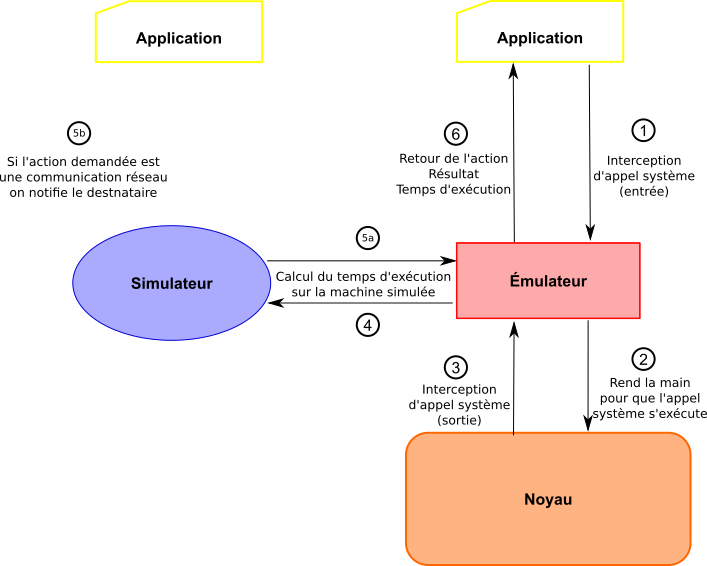
\includegraphics[scale=0.5]{Pictures/png/Emulation_fonctionnement}
   \caption{Fonctionnement de l'émulation par interception.}
   \label{INTERCEPTION}
 \end{figure}
 
 Une application distribuée peut vouloir interagir avec son environnement soit
 pour effectuer de simples calculs, soit pour effectuer des communications avec
 d'autres applications sur le réseau. Quand l'émulateur intercepte une
 communication venant d'un des processus d'une application, il modifie les
 caractéristiques de la communication pour qu'elle puisse s'exécuter sur la
 machine hôte. Il fait la même chose lorsque cette dernière envoie une réponse à
 l'application. En parallèle, l'émulateur demande au simulateur de calculer le
 temps d'exécution de l'action dans l'environnement virtuel pour l'action
 demandée par l'application. L'émulateur envoie ce temps à l'application en plus
 du résultat du calcul demandé pour mettre à jour son horloge. Ainsi, les
 calculs sont réellement exécutés sur la machine, les communications réellement
 émises sur le réseau géré par le simulateur et c'est le temps de réponse qu'il
 fourni qui va influencer l'horloge de l'application. Finalement, les
 applications ne communiquent plus directement entre elles.

 
Pour intercepter ces actions, il faut d'abord choisir à quel niveau se placer.
En effet, une application peut communiquer avec le noyau via différentes
abstractions, Figure \ref{AS_Communication}. Elle peut soit utiliser les
fonctions d'interaction directe avec le noyau que sont les appels systèmes, soit
utiliser les différentes abstractions fournies par le système d'exploitation:
bibliothèques (fonctions de la libc par exemple) ou les fonctions POSIX dans le
cas d'un système UNIX.

Nous allons donc voir comment on peut intercepter et modifier des actions au
niveau de l'application (fichier source puis binaire), des appels système et
des appels de fonctions. Par la suite nous appelerons médiation l'ensemble des
modifications effectuées par l'émulateur sur les actions interceptées.

\begin{figure}[H]
 \centering
 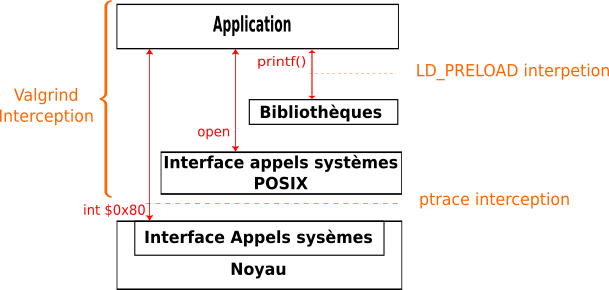
\includegraphics[scale=0.75]{Pictures/png/Communication_application_noyau_v3.png}
 \caption{Communications possibles entre le noyau et une application.}
 \label{AS_Communication}
\end{figure}

\subsubsection{Action sur le fichier source}
\label{section:source}
%% reimplem SMPI (trop spé) ,source to source/ pass LLVM( gcc+libc=consanguin) 
%% , Coccinelle
Le premier niveau auquel on peut se placer pour intercepter les actions est le fichier source de l'application. On peut avant de compiler le code réécrire les parties qui nous intéressent.

Un premier outil pour cela est le programme Coccinelle \citep{cocci}. Il permet de trouver et transformer automatiquement des parties spécifiques d'un code source C. Pour cela, Coccinelle fournit le langage SmPL\footnote{Semantic Patch Language} permettant d'écrire les patchs sur lesquels il va se baser pour transformer le code. Un patch contient une suite de règles, chacune transforme le source en ajoutant ou supprimant du code. Lors de son exécution, Coccinelle scanne le code et cherche les lignes qui remplissent les conditions des règles spécifiées dans le patch et applique les transformations correspondantes. Dans notre cas, il s'agirait de toutes les actions de communications directes ou indirectes avec le noyau susceptibles de mettre à jour l'environnement virtuel. Néanmoins, il ne faut pas oublier de définir une règle pour chacune de ces actions sinon l'interception sera contournée. De plus, il faut pouvoir accéder au fichier source pour le modifier, or cela n'est pas toujours possible.

Une seconde solution beaucoup plus spécifique est de réimplémenter totalement la bibliothèque de communications utilisée par l'application. Cette approche est par exemple utilisée par le projet SMPI\footnote{Simulation d'appplications MPI} \citep{SMPI, clauss2011single}, qui réimplémente le standard MPI au dessus du simulateur SimGrid. Cette approche manque de  généricité car ce travail est à refaire pour chaque bibliothèque de communication existante. 


\subsubsection{Action sur le binaire}
%%Valgrind (perf pourrie)
Pour agir sur le binaire d'une application, c'est l'outil d'instrumentation
d'analyse dynamique Valgrind \citep{Valgrind, Valgrindweb} que nous allons étudier. À l'origine, il est utilisé
pour le débuguage mémoire, puis il a évolué pour devenir l'instrument de base à
la création d'outils d'analyse dynamique de code, tels que la mise en évidence
de fuites mémoires ou le profilage\footnote{Méthode visant à analyser le code
  d'une application pour connaître la liste des fonctions appelées et le temps
  passé dans chacune d'elles}. Valgrind fonctionne à la manière d'une machine
virtuelle faisant de la compilation à volée\footnote{Technique basée sur la
  compilation de byte-code et la compilation dynamique. Elle vise à améliorer la
  performance de systèmes bytecode-compilés par la traduction de bytecode en
  code machine natif au moment de l'exécution}. Ainsi, ce n'est pas le code
initial du programme qu'il envoie au processeur de la machine hôte. Il traduit
d'abord le code dans une forme simple appelée ``Représentation Intermédiaire''. Ensuite, un des outils d'analyse dynamique de Valgrind peut être
utilisé pour faire des transformations sur cette ``Représentation
Intermédiaire''. Pour finir, Valgrind traduit la ``Représentation
Intermédiaire'' en langage machine et c'est ce code que le processeur de la
machine hôte va exécuter. De plus, grâce à la compilation dynamique, Valgrind
peut recompiler certaines parties du code d'un programme durant son exécution et
donc ajouter de nouvelles fonctions au code de l'application.

Dans notre cas, on peut utiliser Valgrind pour mesurer le temps passé à faire un
calcul. Ce dernier étant ensuite envoyé au simulateur pour calculer le temps de
réponse dans l'environnement simulé nécessaire à l'émulateur. On pourrait
également l'utiliser pour réécrire à la volée le code des fonctions que
l'émulateur doit modifier pour maintenir la virtualisation. Pour faire cela, il
faut créer un ``wrapper'' pour chaque fonction qui nous intéresse. Un wrapper
Valgrind est une fonction de type identique à celle que l'on souhaite
intercepter, mais ayant un nom différent (généré par les \texttt{macro} de
Valgrind) pour la différencier de l'originale. Pour générer le nom du wrapper
avec les \texttt{macro} de Valgrind on doit préciser la bibliothèque qui
contient la fonction originale.%% et
%% utiliser un Z-encodage\footnote{ Permet de rendre des caractères valides pour
%%   des noms de fonction en C, Z est le caractère d'échappement pour. Par exemple
%%   : Za pour *, Zp pour +, Zc = :,
%%   ... \\ \url{http://valgrind.org/docs/manual/manual-core-adv.html}}. Cette
%% opération est lourde et complexe. De plus, elle nécessite de connaître le nom de
%% la bibliothèque qui contient la fonction qui nous intéresse
Cela implique donc de connaître pour chaque fonction à intecepter le nom de la
librairie qui l'implémente. Cette solution est donc assez contraignante et ses
performances sont assez médiocres d'après l'étude faite par M. Guthmuller lors
de son stage \citep{MARION:Interception}: facteur de 7.5 pour le temps
d'exécution d'une application avec cet outil. Cette perte de performance est due
à la compilation faite en deux phases ainsi qu'au temps nécessaire aux outils de
Valgrind pour modifier ou rajouter du code à l'existant. Cela pourrait être
acceptable, si Valgrind faisait de la traduction dynamique lors de la seconde
phase de sa compilation, nous permettant ainsi d'avoir du code exécutable sur un
autre type de processeur que celui de l'hôte, mais ce n'est pas le cas.

\subsubsection{Médiation des Appels Système}
%% pourquoi: read/write, comm reseau 

En regardant la Fig.\ref{AS_Communication} et les différents niveaux
d'abstractions, le moyen le plus simple pour attraper les actions de
l'application en gérant un minimum de choses est d'intercepter directement les
appels systèmes.  Ces derniers sont constitués de deux parties; la première,
l'entrée, initialise l'appel via les registres de l'application qui contiennent
les arguments de l'appel puis donne la main au noyau. La seconde, la sortie,
inscrit la valeur de retour de l'appel système dans le registre de retour de
l'application, les registres d'arguments contenant toujours les valeurs reçues à
l'entrée de l'appel système, et rend la main à l'application. \textit{Nous
  devons donc bloquer l'application à chaque interception d'une deux parties de
  l'appel système. Nous permettant ainsi de récupérer et modifier les
  informations permettant de maintenir l'environnement simulé avant de lui
  rendre la main, pour pouvoir entrer ou sortir de l'appel système.}

 Dans cette section, nous allons présenter les outils existants qui permettent
 de faire cela.
 
 \paragraph{L'appel système ptrace}\citep{AS:Interception, MARION:Interception}
 , dont la Fig.\ref{PTRACE_FONCTIONNEMENT} illustre le fonctionnement, permet de
 tracer tous les événement désirés d'un processus. Il peut également lire et
 écrire directement dans l'espace d'adressage de ce dernier, à n'importe quel
 moment ou lorsque un événement particulier se produit. De cette façon on peut
 contrôler l'exécution d'un processus. C'est un appel système dont chaque action
 à effectuer est passée sous forme de requêtes en paramètre de l'appel système.

Pour pouvoir contrôler un processus via \texttt{ptrace}, on va créer deux
processus parents via un \texttt{fork}(); un processus appelé ``processus
espionné'' qui exécutera l'application et qu'on souhaite contrôler, et un autre
qui contrôlera le processus espionné, appelé ``processus espion''. Le processus
espionné indiquera au processus espion qu'il souhaite être contrôlé via un appel
système \texttt{ptrace} et une requête \texttt{PTRACE\_TRACEME} puis il
exécutera l'application via un \texttt{exec}(). À la réception de cet appel, le
processus espion notifiera son attachement au processus espionné via un autre
appel à \texttt{ptrace} et une requête \texttt{PTRACE\_ATTACH}. Il indiquera
également sur quelles actions du processus espionné il veut être notifié (chaque
instruction, signal, sémaphore...), définissant ainsi les actions bloquantes
pour le processus espionné. Dans notre cas, ce seront les appels systèmes que
l'on considérera comme points d'arrêts (requête
\texttt{PTRACE\_SYSCALL)}. Ainsi, le processus espion sera donc appelé deux
fois: à l'entrée et à la sortie de l'appel système.

Quand un des processus de l'application voudra faire un appel système, il sera
bloqué avant de l'exécuter et le processus espion qui lui est associé sera
notifié via un appel système \texttt{ptrace}. Ce dernier fera alors les
modifications nécessaires dans les registres du processus espionné pour
conserver la virtualisation de l'environnement. Pour cela il pourra utiliser les
requêtes \texttt{PEEK\_DATA} et \texttt{POKE\_DATA} passées en argument de
l'appel système {\color{red} (à éclaircir)\textbf{ou modifier directement le
    contenu du /proc/id/mem}}. Puis, il rendra la main au processus espionné
pour que l'appel système puisse avoir lieu.%% Au retour de
%% l'appel système le processus espionné sera de nouveau stoppé et un \texttt{ptrace} sera
%% envoyé au processus espion qui remodifiera les informations nécessaires. Puis il
%% rendra la main au processus espionné bloqué qui sortira de son appel système
%% avec un résultat exécuté sur la machine hôte et un temps d'exécution et une
%% horloge fournie par le simulateur.
 Le même fonctionnement est utilisé pour le retour de l'appel
 système. \textit{Le processus espion change simplement le temps d'exécution de
   l'appel système et l'horloge de l'application en utilisant ceux calculés par
   le simulateur.}  Quand un processus espion a fini un suivi, il peut envoyer
 deux types de requêtes au processus espionné: \texttt{PTRACE\_KILL} qui termine
 le processus espionné ou \texttt{PTRACE\_DETACH} qui le laisse continuer son
 exécution.

\begin{figure}
   \centering
   \includegraphics[scale=0.5]{Pictures/png/ptrace_fonctionnement}
   \caption{Attachement d'un processus et contrôle via un espion}
   \label{PTRACE_FONCTIONNEMENT}
 \end{figure}

Néanmoins, pour contrôler un processus, \texttt{ptrace} fait de nombreux
changements de contexte pour pouvoir intercepter et gérer les événements, or
cela coûte plusieurs centaines de cycle CPU. \textit{De plus, il supporte mal
  les processus utilisant du multithreading, et ne fait pas parti de la norme
  POSIX. Ainsi il peut ne pas être disponible sur certaines architectures et son
  exécution peut varier d'une machine à une autre.}

\paragraph{Uprobes}\citep{AS:Interception, MARION:Interception}
%% Non module noyau

%% pour \textit{user-space probes}, quant à lui permet d'insérer dynamiquement des
%% points d'arrêts à n'importe quel endroit dans le code d'une application, dans
%% notre cas les appels systèmes. Pour chaque point d'arrêt, l’utilisateur fournit
%% un handler particulier à exécuter avant ou après l’instruction marquée. Uprobes
%% étant un outil s'exécutant dans le noyau, les handlers doivent être placé dans
%% un module. Pour chaque point d'arrêt géré par Uprobes, le module noyau contient
%% le handler à exécuter, ainsi que le processus et l'adresse virtuelle du point
%% d'arrêt. Lorsqu'un point d'arrêt est atteint Uprobes prend la main et exécute le
%% bon handler. Pour savoir qu'un point d'arrêt a été touché, Uprobes utilise
%% Utrace, équivalent de ptrace en mode noyau. Ce dernier permet d'éviter les
%% nombreux changements de contexte et est capable de gérer le
%% multithreading. Utrace peut également être utilisé dans le module gérant un
%% point d'arrêt pour récupérer des informations sur l'application et les données
%% qu'elle utilise.

%% Les deux avantages de cette solution sont qu'elle est rapide et qu'elle a accès
%% à toutes les ressources sans aucune restriction. Mais ce dernier point
%% représente aussi son plus gros défaut de par sa dangerosité. De plus, dans notre
%% cas il ne semble pas judicieux de faire de la programmation noyau via un
%% module dont l'utilisateur devra également gérer le bon chargement.

pour \textit{user-space probes}, quant à lui est une API noyau permettant
d'insérer dynamiquement des points d'arrêts à n'importe quel endroit dans le
code d'une application, dans notre cas les appels systèmes, et à n'importe quel
moment de son exécution.

Il existe deux versions de Uprobes la première est basée sur les ``trace
hook\footnote{\url{http://fr.wikipedia.org/wiki/Hook\_\%28informatique\%29}}''\textbf{{\color{red}citation}}. Cette
solution ne sera pas développée ici car elle est très peu utilisée
\textbf{{\color{red} à vérifier}}.

La seconde, la plus connue, se base sur Utrace, équivalent de \texttt{ptrace} en
mode noyau. Ce dernier permet d'éviter les nombreux changements de contexte, qui
dégradent les performances, et est capable de gérer le multithreading. Dans
cette version, l'utilisateur fournit pour chaque point d'arrêt un handler
particulier à exécuter avant ou après l’instruction marquée. Uprobes étant un
outil s'exécutant dans le noyau, les handlers doivent être placés dans un module
noyau. Ce dernier contient pour chaque point d'arrêt géré par Uprobes le handler
à exécuter, ainsi que le pid du processus concerné et l'adresse virtuelle du
point d'arrêt. Pour gérer un point d'arrêt Uprobes utilise trois structures de
données \textit{i)} \texttt{uprobe\_process} (une par processus controlé),
\textit{ii)} \texttt{uprobe\_task} (autant que le processus contrôlé a de
thread), \textit{iii)} \texttt{uprobe\_kimg} (une pour chaque point d'arrêt
affectant un procesus). Chaque structure \texttt{uprobe\_task} et
\texttt{uprobe\_kimg} sont propres à une structure \texttt{uprobe\_process}. La
fonction \texttt{init}() du module va poser les points d'arrêt et la fonction
\texttt{exit}() les enlevera. Pour cela on utilise respectivement la fonction
\texttt{register\_uprobe} et \texttt{unregister\_uprobe}. Ces deux fonctions ont
pour argument le pid du processus à contrôler, l'adresse virtuelle du point
d'arrêt dans le code et le handler à exécuter quand le point d'arrêt est
atteint. La fonction \texttt{register\_uprobes} va trouver le processus passé en
paramètres en parcourant la liste des structures \texttt{uprobes\_process} ou la
crééra si cette dernière n'existe pas. Ensuite, elle crée la structure
\texttt{uprobe\_kimg}, puis fait appel à Utrace pour bloquer l'application, le
temps de placer le point d'arrêt dans le code de celle-ci. Pour cela, on va
placer avant l'instruction sondée un appel au module contenant le handler à
invoquer, puis on rend la main à l'application en utilisant de nouveau
Utrace. \texttt{unregister\_uprobe} fait de même mais supprime la structure
\texttt{uprobe\_kimg} passée en paramètre au lieu de l'ajouter. De plus, s'il
s'agit de la dernière structure de ce type pour un processus contrôlé, il
supprimera alors la structure \texttt{uprobe\_process} et toutes les
\texttt{uprobe\_task} associées.

Lorsqu'un point d'arrêt est atteint Uprobes prend la main et exécute le bon
handler. Pour savoir qu'un point d'arrêt a été touché, Uprobes utilise de
nouveau Utrace, ce dernier envoyant un signal à Uprobes à chaque fois que le
processus qu'il contrôle atteint un point d'arrêt.

Utrace envoie également un signal à Uprobes quand un des processus contrôlé fait
un appel à \texttt{fork}()/\texttt{clone}(), \texttt{exec}(), \texttt{exit}()
pour que ce dernier créé ou supprime les structures uprobe\_process
concernées. Utrace peut également être utilisé dans le handler gérant un point
d'arrêt pour récupérer des informations sur l'application et les données qu'elle
utilise. De plus, un handler peut également ajouter ou enlever des points
d'arrêts.

Les deux avantages de cette solution sont qu'elle est rapide et qu'elle a accès
à toutes les ressources sans aucune restriction. Mais ce dernier point
représente aussi son plus gros défaut de par sa dangerosité. De plus, dans notre
cas il ne semble pas judicieux de faire de la programmation noyau via un module
dont l'utilisateur devra également gérer le bon chargement.

\paragraph{Seccomp/BPF:}
%% Read only
\label{paragraph:seccomp/bpf}

Seccomp \citep{seccompbpf} est un appel système qui permet d'isoler un processus
en lui donnant le droit d'appeler et d'exécuter qu'un certain nombre d'appels
systèmes: \textit{read}, \textit{write}, \textit{exit} et \textit{sigreturn}. Si
le processus fait un autre appel système, il sera arrêté avec un signal
\texttt{SIGKILL}. Comme cela est assez contraignant, le nombre d'applications
que l'on peut utiliser avec seccomp est donc très limité. Pour plus de
flexibilité, on peut utiliser une extension de cet appel système appelée
seccomp/BPF, pour \textit{seccomp BSD Packet Filter}, permettant de définir dans
un programme BPF \citep{BPF_mccanne1993bsd} les appels systèmes autorisés à
s'exécuter, en plus de ceux cités précédemment. Cette dernière fonctionne sur le
même principe que le filtrage de paquet réseau où on établit une suite de
règles. Pour pouvoir s'exécuter, un appel système doit pouvoir passer à travers
toutes les règles. Dans le cas où les appels systèmes \texttt{fork}() ou
\texttt{clone}() peuvent s'exécuter, l'arborescence de filtres est transmise aux
enfants, de même que pour les processus faisant des appels \texttt{execve}()
quand ils sont autorisés. Les règles des filtres BPF portent sur le type de
l'appel système et/ou ses arguments. Ainsi, à chaque entrée ou sortie d'un appel
système, ne faisant pas partie des quatre autorisés par seccomp, l'extension
utilisant BPF est appelée. Elle reçoit en entrée le numéro de l'appel système,
ses arguments et le pointeur de l'instruction concernée. En fonction des règles,
elle laisse l'appel système s'exécuter ou pas.  De plus, seccomp/BPF possède une
option qui lui permet de générer un appel système \texttt{ptrace}(). Cela permet
au processus espion, s'il existe, de ne plus attendre sur chaque appel système
du processus espionné, mais uniquement sur les appels systèmes qu'il souhaite
intercepter.

Néanmoins, l'appel système seccomp et son extension seccomp/BPF ne sont
disponibles que si le noyau est configuré avec l'option \texttt{CONFIG\_SECCOMP}
pour la première et \texttt{CONFIG\_SECCOMP\_FILTER} pour la deuxième. Pour
pouvoir créer des filtres, il faut également avoir des droits particuliers,
notamment l'exécution de certaines commandes root. Ainsi, l'utilisation de cet
appel système et de son extension demande une certaine configuration noyau et
des privilèges pour les utilisateurs, ce qui n'est pas très conseillé.

De plus, si on l'utilise sans l'option d'appel à \texttt{ptrace} on ne peut que
lire le contenu de l'appel système et pas le modifier. On ne peut donc pas faire
de médiation avec cet outil sans faire appel à \texttt{ptrace}. Néanmoins,
l'utilisation de seccomp/BPF avec \texttt{ptrace} permet de réduire
signifiquativement le nombre d'événement sur lequel attendra le processus
espion.
\newline
Malgré ses défauts, l'appel système \texttt{ptrace} semble être le meilleur
outil pour faire ce type d'interception. 

%%avec \textbf{ptrace} ne sont pas possibles, d'où l'alliance
%%   avec LD\_PRELOAD} Par exemple lors d'un gettimeofday l'appel système n'est pas
%% lancé on répond directement au niveau de la bibliothèque ainsi on n'arrive même
%% pas au niveau de l'appel système, donc ptrace ne fait rien.  Problème
%% portabilité {\color{red} \textbf{gérer cette transition}}

\subsubsection{Médiation directe des appels de fonctions}
%%pourquoi: pthread, temps

Puisque l'interception des actions d'une application au plus bas niveau ne
suffit pas, on peut penser qu'une bonne solution est d'intercepter les actions
de l'application au plus haut niveau que sont les bibliothèques. Pour cela nous
allons étudier deux approches basées sur l'éditeur de liens dynamiques de Linux
qui permet d'insérer du code dans l'exécution d'un programme.

\paragraph{LD\_PRELOAD:}
\label{paragraphe:LDPreload}
%pas suid

L'utilisation de la variable d'environnement \texttt{LD\_PRELOAD}
\citep{LDPreload}, contenant une liste de bibliothèques partagées, va nous
permettre d'intercepter les appels aux fonctions qui nous intéressent et d'en
modifier le comportement. Cette variable est utilisée à chaque lancement d'un
programme par l'éditeur de liens pour charger les bibliothèqes partagées qui
doivent être chargées avant toute autre bibliothèque (même celles utilisées par
le programme). Ainsi, si une fonction est définie dans plusieurs bibliothèques
différentes, celle utilisée par le programme sera celle qui est contenue dans la
bibliothèque partagée apparaîssant en premier dans la liste des bibliothèques
préchargées. Ce ne sera pas \textit{nécessairement} celle de la bibliothèque
attendue par le programme. Par exemple, on créé une bibliothèque partagée qui
implémente une fonction open() de même prototype que la fonction open() de la
libc et on place cette bibliothèque dans la variable \texttt{LD\_PRELOAD}. Quand
on exécute un programme faisant un appel à open(), l'éditeur de lien va d'abord
charger les bibliothèques contenues dans la variable d'environnement
\texttt{LD\_PRELOAD} puis la libc, la nouvelle bibliothèque apparaîtra donc
avant la libc dans la liste des bibliothèques préchargées. Ainsi, c'est la
nouvelle fonction open() qui sera exécutée par le programme et non
l'originale. De cette façon, on peut intercepter n'importe quelle fonction.

Dans notre cas, on va donc créer notre propre bibliothèque de fonctions. Pour
chaque fonction susceptible d'être utilisée par l'application, on crééra une
fonction de même nom et de même type dans notre bibliothèque. Chacune de nos
fonctions contiendra alors toutes les modifications nécessaires pour maintenir
notre environnement simulé suivi d'un appel à la fonction initiale. On rappelle
que dans notre cas, on souhaite juste intercepter l'appel et pas l'empêcher.
%%Pour faire
%% appel à la fonction initiale on ne peut pas simplement l'appeler par son nom
%% puisque ce serait notre nouvelle fonction qui serait appelée. On va donc utiliser
%% dans notre nouvelle fonction les fonctions de la famille dlopen, notamment
%% dlopen et dlsym. La première permet de charger une bibliothèque dynamique dont
%% le nom est passé en paramètre et de récupérer un
%% ``handle''\footnote{http://pubs.opengroup.org/onlinepubs/009695399/functions/dlopen.html
%%   \\ A successful dlopen() shall return a handle which the caller may use on
%%   subsequent calls to dlsym() and dlclose(). The value of this handle should not
%%   be interpreted in any way by the caller.} utilisé par dlsym pour trouver
%% l'adresse de la fonction originale qui nous intéresse en mémoire, nous
%% permettant ainsi d'y faire appel.
Notre nouvelle bibliothèque sera préchargée avant les autres en la plaçant dans
la variable \texttt{LD\_PRELOAD}, ainsi nos fonctions passeront avant les
fonctions des bibliothèques usuelles.

Néanmoins, si l'application fait un appel système directement sans passer par la
couche \textit{Bibliothèques} (Fig.~\ref{AS_Communication}) notre mécanisme
d'interception est contourné. \textit{En effet on ne peut surcharger que des
  fonctions définies dans bibliothèques avec cette solution, pas les appels
  systèmes directement.} De même, si on oublie de réécrire une fonction d'une
des bibliothèques utilisée par l'application. Cette solution n'est donc pas
suffisante pour le modèle d'interception que nous souhaitons avoir.

Cependant, on peut voir que \texttt{LD\_PRELOAD} résout les lacunes de
\texttt{ptrace} concernant les fonctions de temps et le multithreading. À
l'inverse, puisque \texttt{ptrace} permet d'intercepter les appels systèmes que
le modèle d'interception avec \texttt{LD\_PRELOAD} ne permet pas de gérer, on
peut dire que \texttt{ptrace} résout les problèmes de \texttt{LD\_PRELOAD}. Une
solution choisie lors d'un précédent stage est donc d'allier les deux. On
surchargera les fonctions temporelles dans notre bibliothèque préchargée avec
\texttt{LD\_PRELOAD} pour pallier les lacunes temporelles de
\texttt{ptrace}. \textit{Et ce dernier s'occupera de toutes les autres
  fonctions}, ainsi on est certain de n'oublier aucune fonction.

\paragraph{Got injection:}
%% plus dur que nécessaire

Dans cette section, nous avons présenté différentes approches permettant de faire de l'interception et de la médiation d'actions d'applications, résumé dans la table \ref{TAB_COMP}. Dans le cas d'émulateur ne souhaitant pas modifier le code source d'une application les outils présentés en \ref{section:source} sont inutiles. De plus, de par le surcoût d'utilisation de Valgrind, cette solution est à écarter dans le cas d'applications distribuées large échelle s'exécutant dans un environnement distribué.

\begin{table}[h]
\resizebox{\textwidth}{!}{%
\begin{tabular}{c|c|c|c|c|c|c|}
\cline{2-7} & \texttt{ptrace} & Uprobes & seccomp/BPF & \texttt{LD\_PRELOAD} &
got Poisoning & Valgrind \\ \hline
\multicolumn{1}{|c|}{\begin{tabular}[c]{@{}c@{}}Niveau
    \\ d'interception\end{tabular}}
& \begin{tabular}[c]{@{}c@{}}Appel\\ Système\end{tabular}
    & \begin{tabular}[c]{@{}c@{}}Appel\\ Système\end{tabular}
        & \begin{tabular}[c]{@{}c@{}}Appel\\ Système\end{tabular} & Bibliothèque
            & Bibliothèque & Binaire \\ \hline \multicolumn{1}{|c|}{Coût} &
            Moyen & Faible(?) & ? & Faible & ? & Important \\ \hline
            \multicolumn{1}{|c|}{Utilisation}
            & \begin{tabular}[c]{@{}c@{}}Assez\\ complèxe\end{tabular} & ? & ? &
                Simple & ? & Complèxe \\ \hline
\end{tabular}
}
\caption{Comparaison des différentes solutions d'interception entre une
  application et le noyau}
\label{TAB_COMP}
\end{table}


\newpage
\textbf{INTRO TODO}

\subsection{CWRAP}
%% pourquoi (tester samba), comment (LD\_PRELOAD comm, suid)

cwrap\citep{cwrap, cwrap_bis} a pour but de tester des applications réseaux s'exécutant sur des machines UNIX ayant un accès réseau limité et sans droits root. Ce projet libre a débuté en 2005 avec le test du framework ``smbtorture'' de Samba\footnote{\url{https://www.samba.org/} \\ \url{https://wiki.samba.org/index.php/Writing\_Torture\_Tests}} Pour atteindre son objectif cwrap fait de l'émulation par interception basée sur le préchargement de quatre bibliothèques via \texttt{LD\_PRELOAD}, comme nous l'avons vu en \ref{paragraphe:LDPreload}.

La première \texttt{socket\_wrapper} gère les communications réseaux. Elle modifie toutes les fonctions liées aux sockets afin que toutes les communication soient basées sur des sockets UNIX et que le routage soit fait sur le réseau local émulé. Cela permetde pouvoir lancer plusieurs instances de serveur sur la même machine hôte. On peut également utiliser les ports privilégiés (en dessous de 1024) sans avoir les droit root dans le réseau local émulé pour communiquer. Cette bibliothèque permet aussi de faire des captures de trace réseau. La seconde \texttt{nss\_wrapper} est utilisée dans le cas d'application dont les démons doivent pouvoir gérer des utilisateurs. Pour cela elle va modifier le contenu des variables d'environnement spécifiant les fichiers passwd et group qui vont être utilisés par l'application pendant la phase de test. Par défaut, les variables contiendraient les fichiers passwd et group du système mais dans ce cas le démon ne pourrait pas les modifier. \texttt{nss\_wrapper} permet également de fournir un fichier host utilisé pour la résolution de noms lors de communications entre sockets. La troisième bibliothèque appelée \texttt{uid\_wrapper} permet de simuler des droits utilisateurs. Autrement dit, elle fait croire aux applications qu'elles s'exécutent avec des droits qui ne sont pas les leurs, par exemple une exécution avec des droits root. Pour cela, on intercepte les appels de type setuid et getuid et on réécrit le mapping fait entre l'identifiant de l'appelant et celui passé en paramètre pour le remplacer par un identifiant possédant les droits désirés. La dernière libraire \texttt{resolv\_wrapper} gère les requêtes DNS. Elle intercepte ces requêtes et soit les redirige vers un serveur DNS de notre choix spécifié dans resolv.conf, soit utilise un fichier de résolution de noms que l'on a fourni à l'application.

Ainsi on a un système complet d'émulation permettant de tester des applications utilisant des réseaux complexes. Le seul bémol étant qu'on utilise uniquement \texttt{LD\_PRELOAD} pour cette émulation, il ne faut donc pas oublier une seule fonction.





\subsection{RR}
\label{subsection:RR}
%% pourquoi (tester firefox), comment (ordre des threads -> perf API dans le CPU)

La plus grande partie de l'exécution d'une application est
déterministe. Néanmoins, il reste des instructions non déterministes entraînant
un exécution toujours différente de l'application (signaux, adresses de
buffers...). Elles peuvent conduire à des fautes qui sont persistantes ou qui
apparaissent après un certain nombre d'exécutions ou qui sont totalement
aléatoires et peuvent ne pas réapparaître lors de la réexécution de
l'application. Essayer de résoudre ces bugs de façon conventionnelle étant très
difficile, il faut trouver de nouvelles méthodes. C'est pour cela que RR a été
créé. RR \citep{RR} est outil de débogage utilisant l'émulation par interception
et qui vise à surpasser gdb. Il a été créé pour déboguer Firefox, mais il
peut-être utilisé sur n'importe quel type d'application. Il résout le problème
des exécutions non déterministes en deux phases. La première consiste à
enregistrer l'exécution de tous les événements non déterministes qui pourraient
échouer. La seconde débogue l'exécution de façon déterministe en rejouant
l'enregistrement aussi souvent qu'on le souhaite. On relance toujours la même
exécution et les ressources restent les mêmes (espace d'adressage, contenu
des registres, appels système), d'où l'idée de déterminisme. Avec cette
méthode, on peut même déboguer les fautes qui sont produites par des outils de
fuzzing\footnote{ Technique pour tester des logiciels basée sur l'injection des
  données aléatoires dans les entrées d'un programme. Si le programme échoue:
  plantage ou génération d'erreur, alors il y a des défauts à
  corriger. \\ \url{http://fr.wikipedia.org/wiki/Fuzzing}} ou d'injection de
fautes. Néanmoins, pour des raisons d'efficacité RR ne sauvegarde pas la mémoire
partagée lors d'exécutions multi-thread. Ce choix permet de n'émuler qu'une
machine mono-c\oe ur qui est plus simple à gérer même si cela empêche le
parallélisme.

RR utilise différents outils selon la phase de son
exécution\citep{RRimplem}. Dans la phase d'enregistrement, pour gérer
l'ordonnancement lors du rejeu, il sauvegarde les actions qu'il considère comme
mécanisme d'interruption d'une application: \textit{i)} les appels système
exécutés \textit{ii)} la préemption via HPC\footnote{Hardware Performance
  Counters \\ On compte les instructions qui s'exécutent et on arrête
  l'application quand le nombre d'instrucions exécuté atteint la valeur du HPC
  fournie par l'utilisateur.} en sauvegardant le nombre d'instructions à exécuter
avant une interruption \textit{iii)} les signaux UNIX exécutés ainsi que leur
handler s'il est réimplémenté. Dans la phase de rejeu, RR utilise les données
non déterministes sauvegardées lors de la première phase pour mettre en place
son émulation (appels système, compteur d'instructions, handler de signal,
valeur des registres lors de ces actions). Quand RR va rejouer un appel système,
les valeurs de retour des registres seront celles sauvegardées lors de
l'exécution réelle et non celles du rejeu. Pour intercepter les appels système,
RR utilise \texttt{LD\_PRELOAD} (section \ref{paragraphe:LDPreload}) qui va les
placer dans un buffer. Ensuite Seccomp/BPF(section\ref{paragraph:seccomp/bpf})
parcourra le buffer pour filtrer les appels système et les laisser
exécuter. Pour cette partie de la gestion de l'appel on n'utilise pas ptrace car
il est trop couteux en terme de changement de contexte, Figure \ref{AS_RR}.
\begin{figure}
\centering 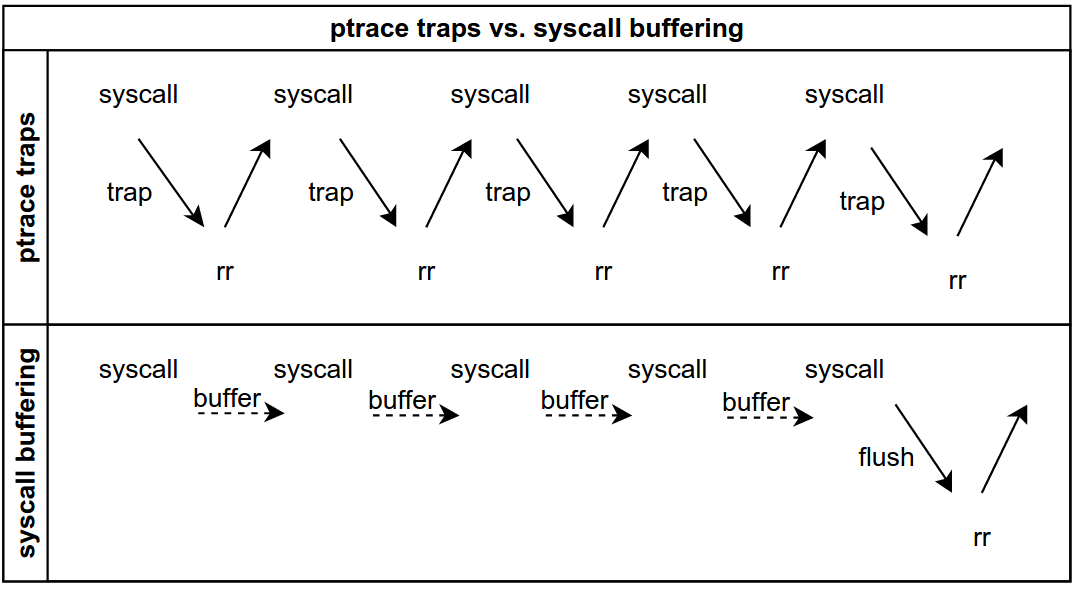
\includegraphics[scale=0.30]{Pictures/png/RR_AS}
\caption{Comparaison de l'exécution du rejeu de RR avec ptrace et seccomp-bpf
  pour gérer l'exécution des appels système.}
\label{AS_RR}
\end{figure}
Il sera utilisé pour renvoyer le bon résultat à l'application (celui sauvegardé
lors de la première phase) et gérer les autres événements de l'application
notamment les signaux et les HPC. Pour pouvoir déboguer l'application on va
utiliser les commandes gbd (placer les points d'arrêts, cotinuer
l'exécution...). En utilisant gdb à l'intérieur de son outil de débogage, RR
veut essayer de le surpasser en terme d'efficacité.

De par son fonctionnement, RR permet donc de diminuer le temps de débogage. De
plus, il peut fonctionner avec de nombreuses applications puisqu'il arrive à
gérer une grosse application telle que Firefox. Le surcoût de la phase
d'enregistrement par rapport à un simple debogage avec gdb varie selon les
applications et les tests effectués. Néanmoins, le fait que RR n'enregistre pas
la mémoire partagée en multi-tâche est un problème pour déboguer des threads. De
plus, il émule une machine simplement mono-c\oe ur ce qui est un problème pour
l'utilisation du parallélisme. Tous les appels système ne sont pas encore
implémentés et en fonction de l'application à tester on risque de voir
apparaître un problème d'interception de certains appels système exécutés par
les processus.

\subsection{Distem}
%Partie virtualisation standard

Distem \citep{DISTEM} est un outil libre permettant de construire des
environnements expérimentaux distribués virtuels. Pour cela il fournit un
système de virtualisation de n\oe uds, une émulation des c\oe urs du processeur
de la machine hôte et du réseau. À partir d'un ensemble de n\oe uds homogènes,
il peut émuler une plateforme de n\oe uds hétérogènes connectés via un réseau
lui-même virtuel.

Cet outil qui se veut simple d'utilisation propose différentes interfaces selon
les besoins et la ???\textit{c quoi le mot que je cherche!!!} de
l'utilisateur. De plus, il supporte parfaitement le passage à l'échelle
puisqu'en 2014 40 000 n\oe uds ont été émulés en utilisant moins de 170 machines
physiques \citep{DISTEM_buchert2014emulation}. Le prochain objectif étant de
réussir à émuler 100 000 machines.

Pour construire un environnement distribué virtuel Distem utilise la
virtualisation par limitation telle que nous l'avons définie dans la section
\ref{section:limitation}. On commence par spécifier la latence et la bande
passante en entrée et en sortie de chaque lien du réseau virtuel. Ensuite, on
définit les performances de chaque n\oe ud émulé. Autrement dit, et c'est ce que
montre la Fig.\ref{Distem_core}, on va allouer à chaque n\oe ud virtuel un
certain nombre de c\oe urs du processeur de la machine physique dont on pourra
controller la fréquence individuellement.

  \begin{figure}[H]
  \centering
  \includegraphics[scale=0.70]{Pictures/png/Distem_repartion_coeurs_v1}
  \caption{Répartition des c\oe urs d'un processeur d'une machine hôte entre les différents noeuds virtuels qu'elle héberge et émulation de leur puissance en utilisant qu'une partie de leur puissance.}
  \label{Distem_core}
  \end{figure}
  
On finit par construire l'environnement de test en plaçant les n\oe uds virtuels sur une machine physique. Pour que l'environnement de test se rapproche au plus près de la réalité, Distem est capable de changer à la volée les paramètres du réseau et la vitesse de chaque c\oe ur alloué à un n\oe ud virtuel.

\begin{figure}
  \centering
  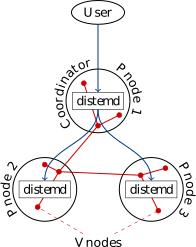
\includegraphics{Pictures/png/Distem_architecture}
  \caption{Architecture de communication de Distem. On a 3 n\oe uds physique (``Pnodes'') contenant chacun 3 n\oe uds virtuels (``Vnodes'')}
  \label{Distem_archi}
\end{figure}

Comme le présente la Fig.\ref{Distem_archi}, Distem repose sur une architecture simple pour construire un environnement de test distribué virtuel : les ``Pnodes'' et les ``Vnodes''. Les premiers sont des n\oe uds physiques non virtualisés alors que les seconds représentent les n\oe uds que l'on souhaite émuler. Un des Pnodes appelé ``coordinator'' gère le contrôle de l'infrastructure dans sa globalité en communiquant avec l'ensemble des Pnodes. Ces derniers peuvent héberger plusieurs Vnodes, chaque Pnode possèdant son démon Distem qui contrôle les Vnodes. Les Vnodes sont séparés et n'ont pas conscience des autres Vnodes présents sur le ``Pnode''. Pour permettre cela, Distem utilise un conteneur LXC pour émuler un Vnode. Ainsi, chaque Vnode possède un espace d'adressage séparé pour les ressources sytème (tâches, interfaces réseau, mémoire...). Néanmoins, les conteneurs LXC partagent l'utilisation du processeur, ainsi on ne peut pas attribuer un certain nombre de c\oe urs de CPU à un Vnode. Pour pallier ce problème, Distem utilise en parallèle le \textit{Linux Control Group{\color{red} todo définir}}. Pour contrôler la puissance des c\oe urs attribués à chaque Vnode, Distem utilise l'algorithme \textit{CPU-Hogs{\color{red} todo définir}} \citep{DISTEM_buchert2011methods}. Ainsi les Vnodes ont conscience les uns des autres uniquement via le réseau virtuel. Chaque Vnodes possède une ou plusieurs interfaces réseau virtuelles reliées au réseau physique de l'hôte afin que les Vnodes puissent communiquer avec l'extérieur. Du fait du grand nombre de n\oe uds qu'on souhaite émuler et qui vont communiquer entre eux cet accès au réseau extérieur pose problème. En effet, pour se reconnaître les n\oe uds vont faire des requêtes ARP et s'ils sont trop nombreux à envoyer ces requêtes en même temps on va se retrouver face à un problème d'ARP flooding. La première solution mise en place par Distem a été d'augmenter la taille des tables ARP pour les Pnodes et les Vnodes ainsi que l'augmentation du \textit{timeout} d'une entrée dans la table. Néanmoins, le but de Distem étant de pouvoir émuler de plus en plus de n\oe uds cette solution ne peut s'appliquer indéfiniment. Une autre solution, qui est celle utilisée actuellement, est de rajouter une couche d'abstraction réseau à l'intérieur du Pnode en utilisant VXLAN\citep{VXLAN_mahalingam2014virtual, DISTEM_buchert2014emulation} comme le montre la Fig.\ref{Distem_VXLAN}. Ainsi, les paquets seront échangés entre Pnodes sur le réseau et c'est la couche VXLAN qui s'occupera d'envoyer au bon Vnodes le paquet reçu sur le Pnodes. Ces derniers étant très peu nombreux on est sûrs de ne pas surcharger les tables ARP.

\begin{figure}
  \centering
  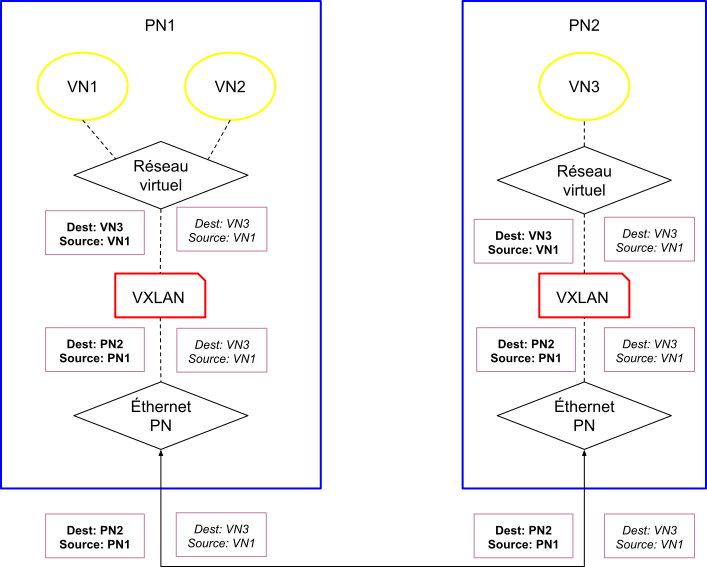
\includegraphics[scale=0.5]{Pictures/png/Distem_VXLAN}
  \caption{Abstractions des communications réseaux de Distem via VXLAN. Les paquets en gras sont ceux envoyés en présence de VXLAN et ceux en italiques sont ceux qui seraient envoyés sur un réseau n'utilisant pas VXLAN}
  \label{Distem_VXLAN}
\end{figure}

On peut donc voir que Distem possède une infrastructure et un réseau émulés bien détaillés et assez réalistes. De plus il est capable de gérer les fautes injectées au niveau des n\oe uds ou sur le réseau. Son seul problème est donc de limiter l'émulation empêchant ainsi l'émulation de machines plus rapides. 

\subsection{MicroGrid}

\subsection{DETER}
\label{subsection:DETER}

Dans le domaine de la cyber-sécurité, le test de solutions de défenses proposées
face aux différentes menaces n'est pas simple et se développe lentement. En
effet, de nombreuses ressources sont nécessaires et il ne semble pas judicieux
d'effectuer les tests en environnement réel. De plus, les innovations qui
fonctionnent parfaitement dans des environnements contrôlés et prédictibles
sont souvent moins efficaces et fiables dans la réalité de par la taille du
réseau et des ressources qui constituent son environnement.  C'est pour cela que
l'USC\footnote{University Southern California} et l'UC
Berkeley\footnote{Université de Californie à Berkeley} ont lancé le projet DETER
\citep{DETER_Project, DETER_benzel2011science, DETER_mirkovic2010deter}. À sa
création en 2003, DETER était un projet de recherche avancée visant à
développer des méthodes expérimentales pour les innovations en matière de
cyber-sécurité (contrer les cyber-attaques, trouver les failles réseaux
...). Puis en 2004, le besoin de tester ces méthodes se faisant de plus en plus
sentir, le développement de DeterLab\footnote{DeterLab: cyber DEfense Technology
  Experimental Research Laboratory} a été lancé. Cette plateforme d'émulation
par interception libre et partagée fournit un environnement de test large
échelle et réaliste. Elle permet également d'automatiser et de reproduire des
expériences pouvant être de différentes natures. En effet, DeterLab peut
\textit{i)} observer et analyser le comportement de cyber-attaques\footnote{
  Attaques DDos et botnets, vers et codes malicieux, protocoles de stockage
  anti-intrusion (intrusion-tolerant), ainsi que le chiffrement et la détection
  de \textit{pattern}.} et de technologies de cyber-défense, \textit{ii)} tester et
mesurer l'efficacité des solutions de défenses proposées pour contrer les
menaces. Les utilisateurs accèdent aux machines dont ils ont besoin pour leurs
expériences, demandent une certaine configuration du réseau, du système et des
applications présente sur les machines. Pour fonctionner, ce laboratoire virtuel a
développé 7 outils complémentaires. Seuls 4 outils nous intéressent dans le cadre de notre projet\footnote{Les 3 autres sont le simulateur de comportement humain DASH, ``Multy-party Experiments'' pour avoir une vision partielle du monde lors d'une expérience et ``Risky Experiment Management Capability'' pour gérer les échanges d'expériences avec le réseau extérieur.}.

Le premier, qui constitue le c\oe ur logiciel et hardware de DeterLab, se base
sur Emulab \citep{EMULAB_INIT}. DeterLab a étendu ce dernier pour permettre de
faire des tests large échelle spécialisés dans le domaine de la cyber-sécurité
et dont la complexité est représentative des réseaux d'aujourd'hui (nombre de
n\oe uds, hétérogénéité des plateformes, contrôle de la bande passante et
délai). Il fournit également une interface web pour gérer à distance ses
expériences, les projets en développement et accéder aux autres outils de
DeterLab.

Pour gérer les ressources nécessaires à leurs expériences, les
chercheurs du projet DETER ont créé ``The DeterLab Containers''
(Figure \ref{Conteneur}). Ces derniers permettent de virtualiser les
ressources et donc de répartir la puissance de calcul là où elle est
nécessaire. Ainsi, pour des ressources nécessitant une machine entière,
le conteneur sera la machine alors que pour une ressource qui n'aura
besoin que d'une partie de la machine, le conteneur sera une
abstraction de cette partie de la machine contenant les ressources
utilisées par l'application. Cela permet d'isoler les tests qui
n'utilisent pas une machine complète et de partager ses ressources
entre plusieurs tests concurrents. Ce mécanisme de virtualisation
s'appelle la ``Multi-resolution Virtualization''.

\begin{figure}
  \centering 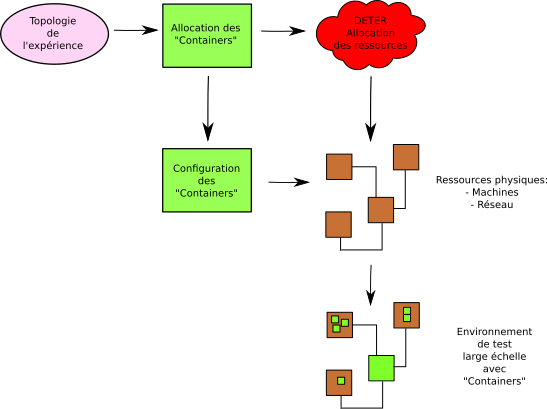
\includegraphics[scale=0.75]{Pictures/png/Deter_fonctionnement_container_v2}
  \caption{Diagramme du fonctionnement d'un \textit{Container}.}
  \label{Conteneur}
\end{figure}

Actuellement, il existe plusieurs plateformes de tests basées sur Emulab avec
des extensions pour pouvoir être utilisées dans des domaines spécifiques comme
le fait DETER. Il se peut qu'une expérience exécutée sur une de ces plateformes
aie besoin de plus de machines que la plateforme ne peut en fournir, que ce soit
en terme de nombre, de puissance ou d'hétérogénéité des machines. Pour pallier
ce problème, le projet DETER a créé la
``Federation''\citep{DETER_faber2007deter}. Elle permet de déployer une
expérience sur plusieurs plateforme de tests différentes et d'avoir un plus
grand facteur de passage à l'échelle. La Figure \ref{Federation} montre
l'exécution d'une expérience dont les 3 n\oe uds sont répartis sur différentes
plateformes. La difficulté ici est que les plateformes sont contrôlées par des
propriétaires différents ayant des règles de sécurité d'accès souvent très
différentes de celles du projet DETER.

-\begin{figure}
  \centering 
\includegraphics[scale=0.75]{Pictures/png/Deter_federation}
  \caption{Fédération d'une experience réparties sur 3 plateformes de tests différentes.}
  \label{Federation}
\end{figure}

Pour que cette solution fonctionne, les plateformes vont partager un système de
nommage permettant de ne pas montrer à l'application la répartition de ses
ressources sur le réseau et une authentification pour contrôler l'accès d'une
plateforme à une autre. Pour gérer cela on va utiliser trois types de n\oe uds
différents (Figure \ref{Federation}). Le premier est le ``federating'', il est
unique et se place sur la plateforme qui demande à exécuter une expérience. Il
cherche les ressources disponibles sur les différentes plateforme puis divise
l'expérience en sous-expérience qu'il assigne à chaque plateforme. Il gère
l'exécution de l'expérience, récupère les données à la fin et
libère les ressources utilisées. Le second type de n\oe ud est le ``federated'',
on en place un sur chaque plateforme. C'est lui qui fournit la liste des
ressources disponibles sur sa plateforme de tests et qui configure les
sous-expériences qu'il reçoit du federating. Il fait la traduction de nom entre
le federating, qui utilise le système de nommage partagé, et le réseau local qui
utilise son système de nommage spécifique.  Il gère également la mise en place
des connexions réseaux entre les entités réparties sur les différentes
plateformes. Le dernier n\oe ud appelé ``local'' est également présent sur
chaque plateforme où l'expérience va s'exécuter. Il gère les communications
entre les différentes plateformes et les sécurise pour éviter les fuites à
l'extérieur du réseau ou l'espionnage par d'autres applications s'exécutant sur
la même plateforme.

Pour finir, MAGI\footnote{Montage AGent Infrastructure} fournit un système de
gestion de flux entre les différentes entités d'une expérience, permettant ainsi
d'avoir un certain contrôle sur les machines. En gérant le flux, on peut
automatiser et reproduire les expériences. En effet, MAGI capture chaque
séquence d'instructions concurrentes que l'expérience va suivre pour gérer le
flux, ainsi on peut rejouer la capture plus tard avec les paramètres d'origine
ou des nouveaux si un fichier de paramètres à tester existe. MAGI permet
également de visualiser l'évolution d'une expérience en cours d'exécution pour
s'assurer que son comportement reste correct sans avoir à attendre le résultat
final. En capturant les configurations demandées par les utilisateurs, MAGI
permet leur réutilisation par d'autres utilisateurs pour éviter à DETER de
reconstruire la même architecture pour une prochaine expérience.

\begin{figure}
\centering
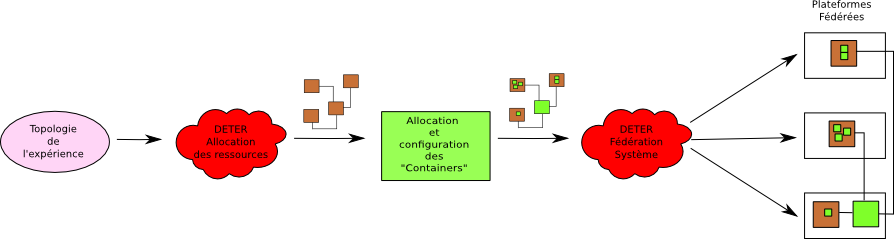
\includegraphics[scale=0.63]{Pictures/png/Deter_fonctionnement_general}
\caption{Création de l'environnement d'une expérience.}
\label{Deter_fonc}
\end{figure}

 Actuellement, DeterLab peut émuler des dizaines de milliers de n\oe uds: le
 projet dispose de 500 machines et 10 FPGA. Il est le seul émulateur dans le
 domaine de la cyber-sécurité et permet de faire des tests large échelle dont la
 complexité est représentative des réseaux.

%% \subsection{ROBOT}


\newpage

\section{Simterpose: Symboles sur lesquels faire de la médiation}
\label{section:simterpose}
Dans le cadre du projet Simterpose de virtualisation légère et de test
d'applications distribuées, c'est l'émulation par interception qui a été
choisi. En effet le but final étant de pouvoir évaluer n'importe quelle
application distribuée sur n'importe quel type d'architecture, on pourrait se
retrouver à devoir émuler des machines plus puissantes que l'hôte, ce que
l'émulation par dégradation ne permet pas. Pour cela on va utiliser SIMGRID
comme simulateur et Simterpose comme émulateur. Simterpose qui est une API de SIMGRID nous permettra donc d'utiliser le simulateur avec des applications
réelles tout en leur faisant croire qu'elles s'exécutent sur des machines
distinctes. Simterpose étant l'émulateur qui va nous permettre d'intercepter les
communications de l'application avec la machine sur laquelle elle s'exécute et
de faire de la médiation nous allons étudier son fonctionnement et voir quels
outils présentés en section \ref{section:emulation} ont été choisis.

\subsection{Organisation générale}
%schéma tableau

\subsection{Les communications réseaux}
 %-> syscall -> ptrace (full mediation, address translation)

Lorsque ptrace est appelé en entrée ou sortie d'appel système, les modifications
à apporter ne sont pas forcément les mêmes selon qu'il s'agit d'une action
nécessitant l'utilisation du réseau ou non. Dans le cas d'un simple calcul ce
qu'il faut maintenir pour l'application, c'est une vision du temps correspondant
à celle qui s'écoulerait si elle était vraiment sur la machine simulée. Ainsi en
entrée d'appel système on n'a pas besoin de modifier quoique ce soit, par contre
au retour il faut modifier le temps d'exécution du calcul en le remplaçant par
celui calculé par le simulateur.

Dans le cas d'une communication réseau, le but de Simterpose étant de réussir à
simuler un réseau réel sur un réseau local, il faut gérer la transition entre
réseau local et réseau simulé. En effet l'application possède une adresse IP et
des numéros de ports ``virtuels'' qui ne correspondent pas forcément à ceux
attribués dans le réseau local. De plus on ne peut pas se baser uniquement sur
le numéro de \textit{file descriptor} associé à une socket pour identifier deux
entités qui communiquent entre elles. En effet ce \textit{file descriptor} est
unique pour chaque socket d'un processus, mais plusieurs processus peuvent avoir
un même numéro de \textit{file descriptor} pour des sockets de communications
différentes puisque chacune à son propre espace mémoire. Pour pallier à ce
problème on va utiliser en plus du numéro de socket, les adresses IP et les
ports locaux et distants des deux entités qui souhaitent communiquer comme moyen
d'identification. Pour gérer toutes ces modifications deux solutions ont été
proposées lors d'un précédent stage
\cite{interception:GUILLAUME:interception_syscall}: la ``médiation par
traduction d'adresse'' et la ``full médiation''.

{\color{red}schéma}
\paragraph{Traduction d'adresse}
 Avec ce type de médiation on considère que le noyau gère des
 communications. Ainsi en entrée et sortie d'appel système Simterpose va juste
 s'occuper de la transition entre réseau ``virtuel'' et réseau local, en
 utilisant les informations de communications contenues dans la socket. Pour
 cela Simterpose gère un tableau de correspondances, dans lequel pour chaque
 couple adresse IP et des ports ``virtuels'', on a un couple adresse IP et ports
 ``réel'' sur le réseau associé.  De fait en entrée d'un appel système de type
 réseau (bind, connect, accept ...), Simterpose devra remplacer l'adresse et les
 ports ``virtuels'' de l'application par l'adresse et les ports réels sur le
 réseau local, ainsi l'appel système se fera avec une source qui existe
 réellement sur le réseau. Au retour de l'appel système il faudra remodifier les
 paramètres en remettant l'adresse et les ports ``virtuels'' pour que
 l'application pense toujours être dans son environnement simulé.  La limite de
 cette approche est liée au nombre de ports disponibles sur l'hôte.

\paragraph{Full médiation} 
Dans ce cas le noyau ne va plus gérer des communications car nous allons
empêcher l'application de communiquer via des sockets et même d'établir des
connexions avec une autre application.  Puisqu'il n'y a aucune communication, on
n'a pas besoin de gérer de tableau de correspondance d'adresse et de ports et
les applications peuvent conserver les adresses et les ports simulées qu'elles considèrent
comme réels. Quand l'application voudra faire un appel système de type
communication ou connexion vers une autre application, le processus espion de Simterpose qui
sera notifié via ptrace neutralisera l'appel système. Ensuite ce processus en
utilisant ptrace récupérera en lisant dans la mémoire du processus espionné les
informations à envoyer ou récupérer et ira directement lire ou écrire ces
informations dans la mémoire du destinataire.  Même si la ``full médiation''
permet d'éviter les communications réseaux et de conserver des tables de
correspondances, dans le cas d'applications qui communiquent énormément et
utilisent de grosses données elle s'avère moins efficace. En effet les appels à
la mémoire sont bien plus coûteux que les communications réseaux.

\subsection{Les thread}
 %% syscall clone + libcalls

\subsection{Le temps}
 %% -> syscall (- system wide), VDSO-linker (cross process ou VDSO)

\subsection{DNS}
%% libcalls (ne rien rater), config fake (system wide), intercept 53 ( plus dur que nécessaire, port dns autre ou pas)

\subsection{Organisation générale}
%schéma tableau

Dans le cadre du projet Simterpose de virtualisation légère et de test
d'applications distribuées, c'est l'émulation par interception qui a été
choisie. En effet, le but final étant de pouvoir évaluer n'importe quelle
application distribuée sur n'importe quel type d'architecture, on peut se
retrouver à devoir émuler des machines plus puissantes que l'hôte, ce que
l'émulation par dégradation ne permet pas. Ce choix exclut donc l'utilisation de
Distem dans notre projet. Les autres outils de virtualisation par interception
ont été écartées pour des raisons différentes: CWRAP utilise uniquement
\texttt{LD\_PRELOAD} pour intercepter les actions et est spécifique aux
applications réseaux. RR gère le multithread mais pas la virtualisation réseau. MicroGrid utilise une émulation par dilation pour gérer le temps. Dans notre cas, nous voulons faire de l'interception.

Pour satisfaire les besoins de notre projet, il a été décidé de créer un nouvel
émulateur Simterpose. Ce dernier doit être simple d'utilisation et facilement
déployable (simple ordinateur ou cluster).  De plus, il doit permettre
d'exécuter plusieurs instances d'une application sur une même machine et de proposer une large gamme de conditions d'exécutions (simple n\oe ud ou réseau
complexe). Les expériences devant être reproductibles, l'émulateur doit pouvoir
générer des traces pour les rejouer dans le simulateur. La résistance aux
pannes, et le fait de pouvoir fonctionner sans avoir accès au fichier source de
l'application sont également des conditions à satisfaire.

Simterpose utilise la plateforme de simulation SimGrid, dont l'architecture
est représentée (Figure \ref{SimGrid}), pour générer l'environnement virtuel
nécessaire à l'expérience. À sa création en 1999, SimGrid
\citep{CASANOVA:SimGrid} était une plateforme fournissant des outils pour
construire un simulateur afin d'étudier les algorithmes d'ordonnancement en
environnement hétérogène, puis il a évolué \citep{MARTIN:SimGrid} pour devenir
plus générique. Aujourd'hui, c'est devenu une plateforme de simulation
permettant d'évaluer les applications distribuées large échelle s'exécutant dans
des environnements hétérogènes.
 
\begin{figure}[H]
  \centering
  \includegraphics[scale=0.86]{Pictures/png/SimGrid}
  \caption{Architecture de la plateforme SimGrid.}
  \label{SimGrid}
\end{figure}

La Figure \ref{Organisation_generale} présente l'organisation générale de la plateforme de simulation. SimGrid va générer l'environnement virtuel. Simterpose intercepte les
actions de l'application et les modifie pour maintenir l'émulation si
nécessaire cf Figure \ref{Organisation_Simterpose}. Puis, il les laisse
s'exécuter sur la machinie hôte et va interroger SimGrid pour qu'il calcule la
réponse de l'environnement virtuel aux actions de l'application (temps d'exécution, gestion de communications réseaux).

\begin{figure}[H]
  \centering
  %\includesvg{Pictures/svg/Communications_Simterpose_interprocess_v2}
  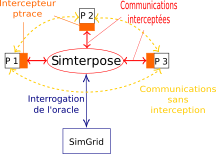
\includegraphics{Pictures/png/Communications_Simterpose_interprocess_v2}
  \caption{Architecture de communication entre les différents acteurs.}
  \label{Organisation_generale}
\end{figure}

\begin{figure}[H]
  \centering
  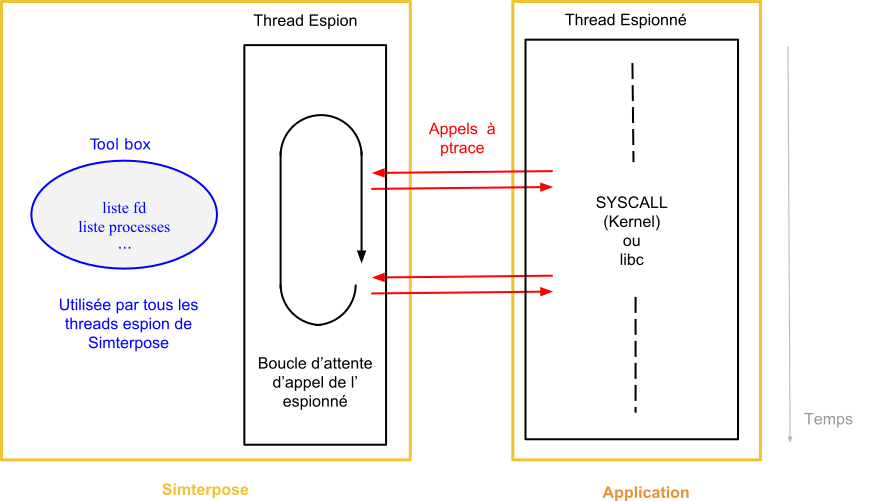
\includegraphics[scale=0.5]{Pictures/png/Simterpose_orga_code_v3}
  \caption{Le fonctionnement de Simterpose.}
  \label{Organisation_Simterpose}
\end{figure}

Maintenant que nous avons présenté le cadre général et l'organisation globale
de notre projet, nous allons nous intéresser au fonctionnement de Simterpose.

\subsection{Les communications réseaux}
 %-> syscall -> ptrace (full mediation, address translation)

Lorsque \texttt{ptrace} est appelé en entrée ou sortie d'appel système, les modifications
à apporter ne sont pas forcément les mêmes dans le cas d'une action nécessitant
l'utilisation du réseau ou non. Dans le cas d'un calcul, il faut simplement
maintenir une vision du temps tel qu'il s'écoule sur la machine simulée pour
l'application. Ainsi en entrée d'appel système on n'a pas besoin de modifier
quoique ce soit, par contre au retour il faut modifier le temps d'exécution du
calcul en le remplaçant par celui calculé par le simulateur.

Dans le cas d'une communication réseau, le but de Simterpose étant de réussir à
simuler un réseau \textit{virtuel} sur un réseau local, il faut gérer la
transition entre réseau local et réseau simulé. En effet l'application possède
une adresse IP et des numéros de ports virtuels qui ne correspondent pas
forcément à ceux attribués dans le réseau local.

\begin{figure}[H]
  \centering
  \begin{subfigure}{0.5\textwidth}
    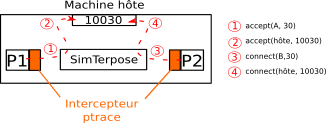
\includegraphics[scale=0.8]{Pictures/png/Mediation_realite}
    \caption{Communications réelles}
  \label{COMM_REALITE}
  \end{subfigure}
  \begin{subfigure}{0.25\textwidth}
  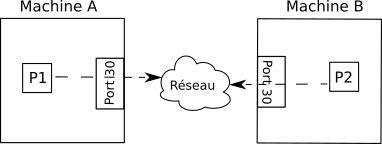
\includegraphics[scale=0.5]{Pictures/png/Mediation_VM}
  \caption{Communications vues \\ par les processus}
  \label{COMM_VM}
  \end{subfigure}
  \caption{Les communications réseaux entre deux processus}
  \label{COMM}
\end{figure}

De plus on ne peut pas se baser uniquement sur le numéro de \textit{file
  descriptor} associé à une socket pour identifier deux entités qui communiquent
entre elles. En effet ce \textit{file descriptor} est unique pour chaque socket
d'un processus, mais plusieurs processus peuvent avoir un même numéro de
\textit{file descriptor} pour des sockets de communications différentes puisque
chacune à son propre espace mémoire. Pour pallier à ce problème on va utiliser
en plus du numéro de socket, les adresses IP et les ports locaux et distants des
deux entités qui souhaitent communiquer comme moyen d'identification. Pour gérer
toutes ces modifications deux solutions ont été proposées lors d'un précédent
stage \citep{GUILLAUME:Interceptionsyscall}: la \textit{médiation par traduction
  d'adresse} et la \textit{full médiation}.

 \begin{figure}[H]
   \centering
   \begin{subfigure}{0.5\textwidth}
   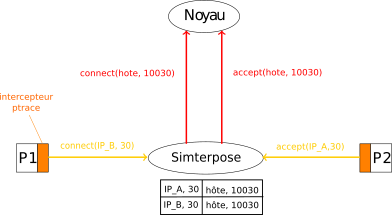
\includegraphics[scale=0.5]{Pictures/png/Mediation_translation_v2}
   \caption{Médiation par traduction d'adresse}
   \label{ADDRESS_TRANSLATION}
   \end{subfigure}
   \begin{subfigure}{0.4\textwidth}
     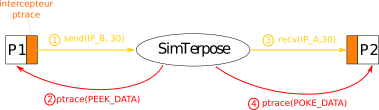
\includegraphics[scale=0.5]{Pictures/png/Mediation_full_v2}
  \caption{Full meditation}
  \label{FULL_MEDIATION}
   \end{subfigure}
   \caption{Les différents types de médiation}
   \label{MEDIATION}
 \end{figure}
 
\paragraph{Traduction d'adresse}
 Avec ce type de médiation, illustrée Fig.\ref{ADDRESS_TRANSLATION}, on considère
 que le noyau gère les communications. Ainsi en entrée et sortie d'appel système
 Simterpose va juste s'occuper de la transition entre le réseau virtuel simulé
 par SIMGRID et le réseau local, en utilisant les informations de communications
 contenues dans la socket. Pour cela, Simterpose gère un tableau de
 correspondances, dans lequel pour chaque couple <IP, ports virtuels> , on a un
 couple <IP, ports réels> associé.  De fait, en entrée d'un appel système de
 type réseau (\texttt{bind}, \texttt{connect}, \texttt{accept} ...), Simterpose
 doit remplacer l'adresse et les ports virtuels de l'application par l'adresse
 et les ports réels sur le réseau local, afin que la source de l'appel système
 corresponde à une machine existante sur le réseau local. Au retour de l'appel
 système, il faudra remodifier les paramètres en remettant l'adresse et les
 ports virtuels pour que l'application pense toujours être \textit{dans un
   environnement distribué.}  La limite de cette approche est liée au nombre de
 ports disponibles sur l'hôte.

\paragraph{Full médiation} 
Dans ce cas, le noyau ne va plus gérer les communications car nous allons
empêcher l'application de communiquer via des sockets et même d'établir des
connexions avec une autre application. Puisqu'il n'y a aucune communication, on
n'a pas besoin de gérer de tableau de correspondance d'adresse et de ports et
les applications peuvent conserver les adresses et les ports simulées qu'elles
considèrent comme réels. Quand l'application voudra faire un appel système de
type communication ou connexion vers une autre application, le processus espion
de Simterpose qui sera notifié via \texttt{ptrace} neutralisera l'appel système,
comme illustré sur la Fig.\ref{FULL_MEDIATION}. \textit{Ensuite, ce processus en
  utilisant \texttt{ptrace} récupérera, en lisant dans la mémoire du processus
  espionné, les données à envoyer ou récupérer et ira directement les lire ou
  les écrire dans la mémoire du destinataire.}  Même si la \textit{full
  médiation} permet d'éviter les communications réseaux et de conserver des
tables de correspondances, elle s'avère moins efficace dans le cas
d'applications qui communiquent énormément et utilisent de grosses données. En
effet, les appels à la mémoire sont bien plus coûteux que les communications
réseau.

 
%% begin{figure}
%%   \centering
%%   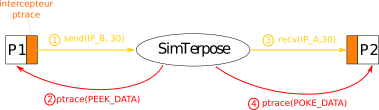
\includegraphics[scale=0.5]{Pictures/png/Mediation_full_v2}
%%   \caption{{\color{red} \textbf{TODO}}}
%%   \label{FULL_MEDIATION}
%% \end{figure}

\subsection{Les thread}
 %% syscall clone + libcalls

\subsection{Le temps}
 %% -> syscall (- system wide), VDSO-linker (cross process ou VDSO)

\subsubsection{DNS}
%% libcalls (ne rien rater), config fake (system wide), intercept 53 ( plus dur que nécessaire, port dns autre ou pas)

Dans le cas d'utilisation du protocole DNS, on peut vouloir modifier le
comportement de l'application afin qu'elle utilise d'autres serveurs que ceux
utilisés par défaut ou aucuns afin que la résolution soit entièrement géré par
Simterpose. Pour gérer cela plusieurs solutions sont envisageables.

Une première solution serait de faire de l'interception de communications au
niveau du port 53, utilisé par défaut dans DNS. Néanmoins, cela est assez
complexe à \oe uvre car il faut pour chaque communication faite par
l'application tester le port qu'elle souhaite utiliser. De plus, il est possible que l'utilisateur définisse un autre port pour le protocole DNS que
celui par défaut. Cette solution n'est donc pas suffisante.

Une autre approche serait de remplacer le fichier \texttt{resolv.conf} utilisé
pour la résolution de nom. Ainsi, l'utilisateur configurerait son propre
fichier, il pourrait égalemment fournir un fichier de spécifications de
comportement en cas d'utilisation de DNS permettant à Simterpose de générer un
nouveau fichier \texttt{resolv.conf}. Néanmoins, cette solution génère une
surcharge de travail pour l'utilisateur or nous souhaitons avoir un émulateur
qui soit simple d'utilisation.

La dernière solution envisageable est de faire de l'interception d'appel de
fonctions. Dans cas, on créé une bibliothèque partagée qui réécrit les foncitons
liés à la résolution de nom que l'on inclut dans la variable d'environnemnt
\texttt{LD\_PRELOAD}. Mais on a toujours le même problème qui est de n'oublier
aucune fonction pour maintenir notre environnement virtuel. Pour l'instant,
c'est la solution qui a été choisie. N'ayant pas encore été mise en place, il
n'est pas exclu que nous devions trouver une autre solution pour gérer le DNS.

\vspace{0.5cm}

Dans cette section, nous avons étudié l'organisation globale de Simterpose. Le
fonctionnement interne de cet émulateur montre la complémentarité de deux outils
présentés en section \ref{section:interception}: l'appel système \texttt{ptrace}
et la variable d'environnement \texttt{LD\_PRELOAD}. En
effet, \texttt{LD\_PRELOAD} résout les lacunes de \texttt{ptrace} concernant les
fonctions de temps et le multithreading. A l'inverse, puisque \texttt{ptrace}
permet d'intercepter les appels systèmes que \texttt{LD\_PRELOAD} ne permet pas
de gérer, \texttt{ptrace} résout donc les problèmes de \texttt{LD\_PRELOAD}.


\newpage
\section{Travail réalisé}
Au cours de ce stage deux fonctionnalités majeures de Simterpose ont été implémentées: le réseau de communication et la gestion du temps. Ces fonctionalités ont parfois nécessité la mise en place de nouvelles fonctionnalités qui n'avaient pas été prise en comptes lors de la création de Simterpose. Dans cette section, nous allons présenter les deux fonctionnalitées implémentées ainsi que les outils qu'elles ont nécessités.

\subsection{Réseau de communications}

\begin{itemize}
\item sys\_file
\item deux mediation pour chaque appel paragraph section précédente
\end{itemize}

\subsection{Temps}
\begin{itemize}
\item paragraph section précédente
\item pourquoi protéger temps simulation
\item deux mediation pour chaque appel pourquoi non
\item nouvel AS pour gérer le temps dans Simterpose
\end{itemize}


\newpage
\section{Évaluation des fonctionalités implémentées}
\label{section:evaluation}
{\color{red} TODO}

\begin{itemize}
\item transition avec section précédente / intro section
\item description architecture de tests
\item description archi reseau de simterpose
\end{itemize}

\subsection{Réseaux}
\label{subsection:res}
\subsubsection{Protocole}
\begin{itemize}
  \item Calcul temps simulation
  \item Plateforme reseux ou pas?
\end{itemize}

Dans la section précédente nous avons présenté l'oganisation du réseau de communications de Simterpose. Après avoir implémenté cette fonctionalité, nous avons souhaité évaluer ses performances à travers divers tests. Pour effectuer nos expériences, nous avons utiliser à chaque fois deux applications réseau d'échanges de messages. La première application consiste à faire communiquer un client et un serveur en envoyant au serveur un million de messages de petite taille. La seconde quand à elle consiste à envoyer depuis un client un message de 1Mo à un serveur. Le protocole pour chaque expérience a été effectuée 20 fois en utilisant les mêmes appels systèmes pour communiquer les messages ({\color{red}sendto/recvfrom et sendmsg/recvmsg}), puis une moyenne du temps d'exécution ainsi qu'une mesure des temps minimum et maximum ont été conservées.

\subsubsection{Overhead conçernant le temps d'exécution}
L'objectif principal étant de montrer qu'il est possible de faire de la virtualisation légère, nous avons d'abord souhaité mesurer l'\textit{overhead} dû à l'utilisation de Simterpose. De cette façon, si le surcoût d'utilisation de notre émulateur est négligeable on pourra conclure que ce type de virtualisation est possible pour le réseau.

Pour cela, nous avons exécutés les deux applications réseaux présentées plus haut sur une machine en utilisant uniquement le réseau local puis en utilisant Simterpose. Ainsi, en comparant les temps d'exécutions des applications sur les deux types d'architecture nous pourrons calculer l'\textit{overhead}. Les résultats de ces expériences sont présentés Figures \ref{Network_Big_Local} et \ref{Network_Little_Local}. Dans le cas de l'envoi de plusieurs petits messages le temps moyens d'exécution en local est d'environ 3 secondes, avec Simterpose on arrive à 72 secondes en \textit{full mediation} et à 75 secondes en \textit{médiation par traduction d'adresse}. On a donc une exécution qui prends 25 fois plus de temps. De même, lors de l'envoi d'un gros message le système met 0,01 secondes en moyenne pour exécuter l'application alors que Simterpose met entre 1 et 1,1 secondes selon le type de médiation. Cette exécution prendra donc 100 fois plus de temps si on souhaite réellement mettre en place notre émulateur.

\begin{figure}
  \centering
    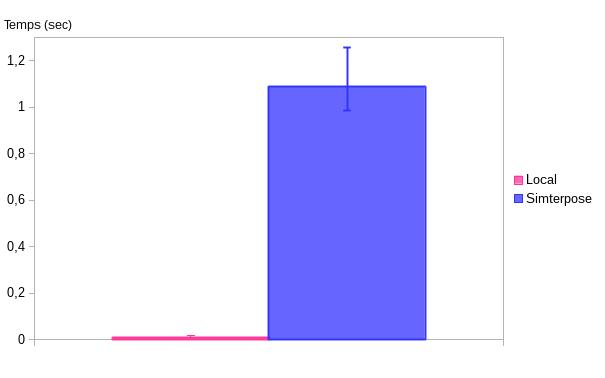
\includegraphics[scale=0.5]{mesures/graph/Bigmsg_local.jpg}
    \caption{Temps d'exécution lors de l'envoi d'un message de 1Mo avec et sans Simterpose.}
    \label{Network_Big_Local}
\end{figure}

\begin{figure}
  \centering
    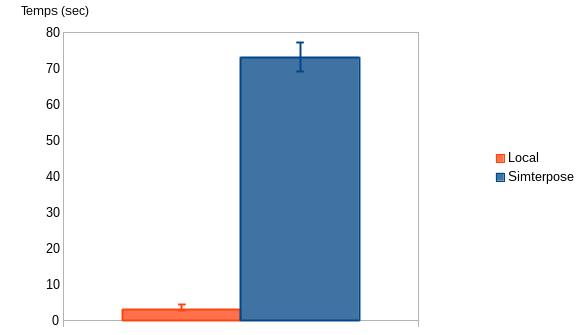
\includegraphics[scale=0.5]{mesures/graph/Littlemsg_local.jpg}
    \caption{Temps d'exécution lors de l'envoi d'un million de messages de 128o avec et sans Simterpose.}
    \label{Network_Little_Local}
\end{figure}
  
Néanmoins, cet écart s'explique par les nombreux appels systèmes et changements de contexte que nécessite Simterpose de par son utilisation coûteuse de ptrace en plus de l'exécution de l'appel système lui-même. Pour la première expérience on peut considérer que cet overhead représente un cas extrême car les utilisateurs en général ne testent pas leurs applications en envoyant des millions de message entre un client et un serveur. De plus, du point de vue humain une exécution 1ms ou 1s dans le second cas ne change pas grand chose pour notre perception. Ainsi, on peut considérer que l'overhead produit par Simterpose sur le temps d'exécution est acceptable.

\subsubsection{Quelle médiation pour quel type d'application}
Dans un second, temps nous avons voulu mesurer les performances des deux types de médiations que nous avons implémentés. Pour cela, nous avons repris le même schéma d'expériences que celui utilisé pour mesurer l'overhead. Les résultats de ces expériences sont présentés Figures \ref{Network_Big_Mediation} et \ref{Network_Little_Mediation}.

Lorsque l'on envoie de nombreux petits messages, on peut constater que la \textit{full mediation} est plus rapide que la \textit{médiation par traduction d'adresse} avec un écart moyen de 3 secondes. Ce résultat s'explique par le fait que lorsqu'on utilise la \textit{médiation par traduction d'adresse} l'envoi de messages génère des appels systèmes et changements de contexte qui n'ont pas lieu en \textit{full mediation} puisque dans ce cas, comme nous l'avons expliqué en section \ref{paragraph:FULL_MEDIATION}, les appels systèmes ne sont pas exécutés. Ces derniers étant couteux cela explique pourquoi la  \textit{médiation par traduction d'adresse} est moins rapide. De plus, en \textit{full mediation}, même si les appels systèmes sont bloqués, nous utilisons l'appel système ptrace pour effectuer nous-même les appels demandés par l'application que nous avons bloqués. Cette méthode même si elle reste moins couteuse que l'exécution de l'appel système demandé consomme des cycles CPU, ce qui explique le faible écart entre les temps d'exécution moyen des deux types de médiation.

Lorsque l'on envoie un gros message, on constate que l'écart moyen entre les deux types de médiations est quasi nul, 0.03 secondes. Nous pensons que dans ce cas la \textit{médiation par traduction d'adresse} est légèrement plus rapide car nous envoyons un seul message de 1Mo de données. En effet, même en \textit{full mediation} on a beaucoup moins de changement de contexte de par le blocage des appels systèmes ici on ne fait qu'un seul appel et la faible différence entre les deux médiations ne peut donc être dû à cela. Par contre, lors de l'envoi d'un tel message il faut prendre en compte la gestion de la mémoire car le message doit être stocké avant de pouvoir être envoyé par morceau sur le réseau. Ainsi, si on ne gère pas la mémoire de façon efficace on surconsomme des cycles CPU. Or, nous n'avons pas encore mis en place de politique de gestion de mémoire particulière pour Simterpose. Néanmoins, si on regarde la largueur des intervalles des temps d'exécution, en \textit{médiation par traduction d'adresse} les temps d'exécution varient bien plus qu'en \textit{full mediation}. On peut donc supposer qu'avec une politique de gestion mémoire aussi efficace que celle qui est utilisée par le système la \textit{full mediation} serait probablement plus rapide que la \textit{médiation par traduction d'adresse} comme dans l'expérience précédente.

\begin{figure}
  \centering
    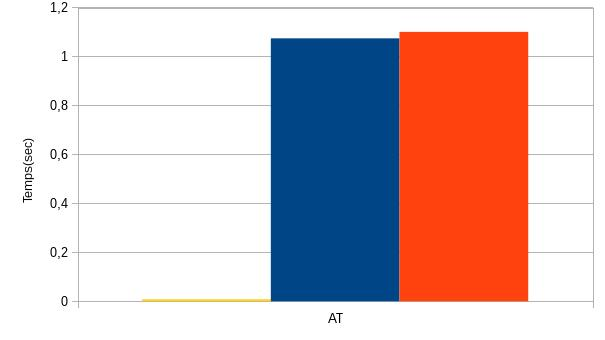
\includegraphics[scale=0.5]{mesures/graph/Bigmsg.jpg}
    \caption{Temps d'exécution lors de l'envoi d'un message de 1Mo avec et sans Simterpose.}
    \label{Network_Big_Mediation}
\end{figure}

\begin{figure}
  \centering
    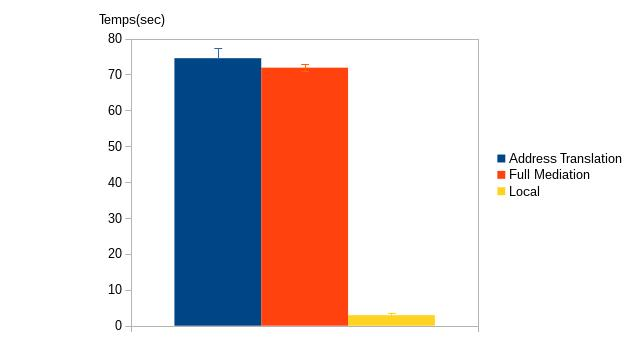
\includegraphics[scale=0.5]{mesures/graph/Littlemsg.jpg}
    \caption{Temps d'exécution de l'envoi d'un million de messages de 128o avec et sans Simterpose.}
    \label{Network_Little_Mediation}
\end{figure}
  
Ces expériences nous ont permis de montrer que lors de l'envoi de nombreux messages il vaut mieux privilégier la \textit{full mediation}. Nous avons également pu voir que pour envoyer de gros messages, les deux médiations se valent. De plus, la faible durée d'exécution d'une expérience nous permet de considérer que l'overhead dû à la mise en place de Simterpose est acceptable. Ainsi, nous pouvons dire que notre implémentation du réseau de communications permet de faire de la virtualisation légère à ce niveau. Nous allons maintenant voir si il en est de même pour une autre fonctionnalité implémentée au cours de ce stage: le temps.

\subsection{Temps}
\label{section:temps}
Dans la section \ref{subsubsection:time}, nous avons pu voir qu'il est important de gérer le temps que l'applciation voit s'écouler. En section \ref{section:work}, nous avons présenté l'implémentation qui a été choisie pour résoudre cette problématique. Maintenant, nous souhaitons mesurer le surcoût ajouté par cette fonctionnalité lors de l'exécution de Simterpose. Si ce surcoût est acceptable, on pourra considérer qu'il est également possible de mettre en place une virtualisation légère qui gère l'écoulement du temps.

\subsubsection{Protocole}
Pour évaluer notre implémentation nous n'allons pas utiliser les mêmes expériences que pour le réseau de communications car le but ici est d'intercepter de les fonctions temporelles et de mesurer le coût de cette interception. Ainsi, nous avons créé une application qui exécute différents appels à des fonctions temporelles (ftime, time, gettimeofday, localtime, mktime...). Le protocole utilisé pour exécuter l'application est également différent. Nos expériences vont ici consister à exécuter 20 fois l'application dans quatre configurations différentes qui soient comparables. Tout d'abord nous allons exécuter l'application qui effectue les appels temporels avec Simterpose en \textit{full mediation} sans LD\_PRELOAD et avec LD\_PRELOAD. Puis, nous ferons de même pour la \textit{médiation par traduction d'adresse}. Les résultats de ces quatres expériences sont présentés Figure \ref{Temps_FM} et \ref{Temps_AT}.

Le changement de médiation ne devrait pas influer sur les performances car chaque médiation intervient uniquement lorsqu'on souhaite effectuer des appels systèmes réseaux que l'on fasse de l'interception avec LD\_PRELOAD ou pas. En comparant les deux graphiques présentés Figure \ref{Temps_FM} et \ref{Temps_AT}, on voit bien que les courbes d'interception via LD\_PRELOAD se superposent et qu'il en est de même pour celle sans interception quelque soit la médiation utilisée. Cela confirme bien l'hypothèse que nous avons fait. Nous pouvons maintenant nous intéresser à l'impact de l'interception sur chaque type médiation.

\subsubsection{Full mediation}
Nous allons d'abord analyser les deux premières expériences, Simterpose en \textit{full mediation} avec et sans intercpetion via LD\_PRELOAD présentées Figure \ref{Temps_FM}. On constate que le temps d'exécution avec interception via LD\_PRELOAD est plus ou moins constant (environ 1,03 secondes), alors que celui sans interception varie énormément, entre 0,82 et 1,13 secondes. Cela est dû au fait que lorsqu'on appelle des fonctions temporelles sans interception via LD\_PRELOAD la bibliothèque VDSO, citée en section \ref{subsubsection:time}, est appelée pour gérer l'appel et accéder elle-même à la mémoire. Cet accès n'a pas un coût constant puisqu'il dépend de la charge du système qui varie en permanence même si on ne fait tourner que notre application et aucune autre en parallèle. Ainsi, le temps d'exécution peut varier comme c'est la cas ici alors qu'il est stable quand on utilise LD\_PRELOAD puisqu'on empèche ces accès. Néanmoins, en moyenne les deux expériences ont environ le même temps d'exécution, 1 seconde pour la première et 1,02 secondes pour la deuxième. On peut donc considérer que l'interception via LD\_PRELOAD a un surcoût négligeable lorsqu'on utilise Simterpose en \textit{full mediation}.

\begin{figure}
  \centering
    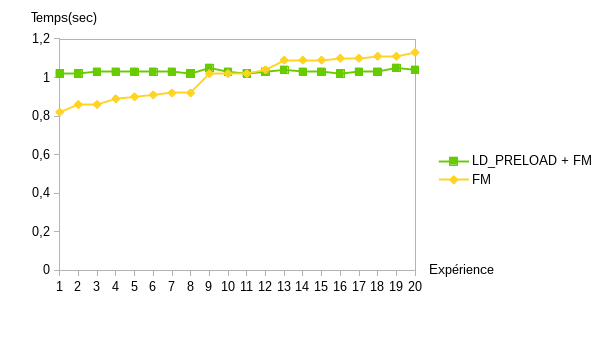
\includegraphics[scale=0.80]{mesures/graph/Temps_FM.png}
    \caption{Temps d'exécution d'une application temporelle en \textit{full mediation} avec interception via LD\_PRELOAD et sans interception}
    \label{Temps_FM}
\end{figure}

\subsubsection{Mediation par traduction d'adresse}
Nous allons maintenant voir s'il en est de même pour les deux dernières expériences, Simterpose en \textit{médiation par traduction d'adresse} avec et sans intercpetion via LD\_PRELOAD, présentées Figure \ref{Temps_AT}. On constate ici aussi que le temps d'exécution avec interception via LD\_PRELOAD est plus ou moins constant (environ 1,02 seconde), alors que celui sans interception varie beaucoup, entre 0,86 et 1,12 secondes. Cela est dû comme précédement à l'utilisation de la bibliothèque VDSO en l'absence d'interception via LD\_PRELOAD. De plus, le temps d'exécution moyen des deux expériences est le même: 1,02 secondes. Dans ce cas, on peut dire que l'interceprtion via LD\_PRELOAD en \textit{médiation par traduction d'adresse} n'a aucun surcoût.

\begin{figure}
  \centering
    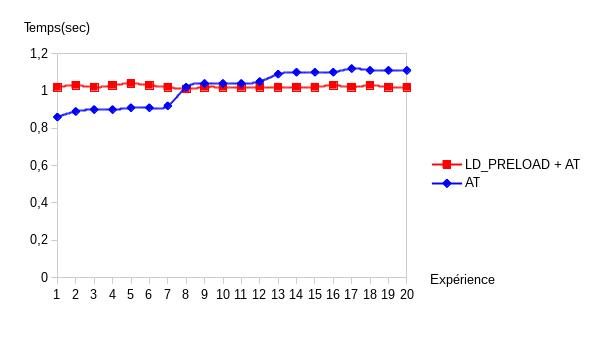
\includegraphics[scale=0.65]{mesures/graph/Temps_AT.jpg}
    \caption{Temps d'exécution d'une application temporelle en \textit{full mediation} avec interception via LD\_PRELOAD et sans interception}
    \label{Temps_AT}
\end{figure}

Ainsi, nous avons pu voir que le surcoût dû à l'interception des fonctions temporelles via LD\_PRELOAD est inexistant en \textit{médiation par traduction d'adresse} et qu'il est négligeable \textit{full mediation} (environ 2\%). On peut donc considérer que nous avons réussi à mettre en place une virtualisation légère qui gère également l'écoulement du temps et qui plus est de façon particulièrement efficace.

\vspace{0.5cm}

{\color{red} \textbf{TODO ccl}}
On peut dire que blabla, d'autres fonctionalites blabla pas necessite d'experiences juste fonctionnelles.



\newpage
\section{Conclusion}
\label{section:ccl}

Dans ce rapport, nous avons présenté notre objectif ainsi qu'un état de l'art
des différentes approches et outils existants. Pour pouvoir exécuter n'importe
quel type d'applications distribuées dans des conditions environnementales qui
permettront de les étudier, la meilleure solution semble être la virtualisation
par interception. Les projets existants ne permettant pas de résoudre les quatre
problèmes engendrés par cette virtualisation (gestion du temps, des threads, des
communications réseaux et le DNS), un nouveau projet a été lancé.

L'émulateur Simterpose dévelopé au LORIA permet d'exécuter et de tester des
applications distribuées réelles, sans disposer de leur code source, dans un
environnement virtuel. Il se base sur la plateforme de simulation SimGrid pour
mettre en place l'environnement d'exécution dans lequel l'application pensera
s'exécuter. Pour maintenir la virtualisation, les actions des applications sont
interceptées et modifiées pour ensuite être exécutées. On utilise SimGrid pour
calculer la réponse de l'environnement virtuel aux différentes actions. La
solution proposée intercepte les actions à deux niveaux différents: appels
systèmes et bibliothèques. Simterpose permet également d'injecter diverses
fautes dans la simulation pour avoir une virtualisation plus réaliste.

Néanmoins, il reste à ajouter certaines fonctionalités (DNS, fonctions de temps)
afin de vérifier qu'il est possible de mettre en place une virtualisation par
inteception qui apporte une réponse à notre problématique. Une fois que nous
aurons un émulateur fonctionnel et complet, nous essayerons d'améliorer son
efficacité. Nous projetons par la suite d'évaluer les performances de notre
projet, afin d'augmenter la taille des expériences.



\newpage

% Bib
\bibliographystyle{plainnat}
\bibliography{src/8.Biblio} % The file containing the bibliography
\label{fin}

\end{document}
